\documentclass[a4paper, 12pt]{article}

%%%%%%%%%%%%
% Packages %
%%%%%%%%%%%%

\usepackage[english]{babel}
\usepackage{packages/sleek}
\usepackage{csvsimple}
\usepackage{booktabs} % for nicer table rules
\usepackage{float}
\usepackage{listings}
\usepackage{xcolor}
\usepackage{inconsolata}  % Nicer monospace font
\usepackage{graphicx} % For including images
\usepackage{subcaption}  % in preamble
\usepackage{enumitem}

\usepackage{tikz}
\usetikzlibrary{arrows.meta, positioning, shapes.geometric}

\lstset{
  basicstyle=\ttfamily\small,        % Smaller monospaced font
  frame=single,                        % No box frame=none
  breaklines=true,                   % Automatic line breaks
  columns=fullflexible,              % Better spacing
  showstringspaces=false,            % Don't show spaces in strings
  tabsize=2,                         % Tabs = 2 spaces
  numbers=left,                      % Line numbers on the left
  numberstyle=\tiny\color{gray},     % Smaller line number style
  captionpos=b,                      % Caption below the code
  keywordstyle=\color{blue},         % Keywords in blue
  commentstyle=\color{gray},         % Comments in gray
  stringstyle=\color{orange},        % Strings in orange
  numbers=none, % No line numbers
}

% Custom style for code listings
\lstdefinestyle{plain}{
    basicstyle=\ttfamily\small,
    frame=none,
    breaklines=true,
    columns=fullflexible,
    showstringspaces=false,
    tabsize=2,
    numbers=none,
}
\lstset{style=plain}


\addbibresource{./resources/bib/references.bib}


\newcommand{\projectTitle}{YouBot Project}
\newcommand{\projectSubtitle}{Inspection, Development and Deployment of the KUKA YouBot Mobile Base}
\newcommand{\authorName}{Aditya Agrawal}
\newcommand{\advisorName}{assistant professor Tomasz Kucner}
\newcommand{\supervisorName}{senior university lecturer Salu Ylirisku}
\newcommand{\courseName}{ELEC-C0302 Final Project in Digital Systems and Design}
\newcommand{\universityName}{Aalto University}


\newcommand{\commentout}[1]{}
\newif\ifshowadi
\showaditrue% Set to \showaditrue to display comments on extending thesis

\newcommand{\adi}[1]{\ifshowadi\textcolor{red}{#1}\fi}

\newif\ifshownotes
\shownotestrue% Set to \shownotestrue to display notes

\newcommand{\notes}[1]{\ifshownotes\textcolor{blue}{#1}\fi}

\newcommand{\code}[1]{\texttt{\detokenize{#1}}}




%%%%%%%%%%%%
% Document %
%%%%%%%%%%%%

\begin{document}

%%%%%%%%%%%%%%
% Title-page %
%%%%%%%%%%%%%%
    \begin{titlepage}
        \raggedright
        % Define variables for title page
        

        \vspace*{2cm}

        {\Huge \textbf{\projectTitle}}\\[0.5cm]
        {\Large \projectSubtitle}\\[2cm]

        \textbf{Author:} \authorName\\[0.3cm]
        \textbf{Advisor:} \advisorName\\[0.3cm]
        \textbf{Supervisor:} \supervisorName\\[2cm]

        \courseName \\
        \universityName\\[0.5cm]
        \today

        \vfill
    \end{titlepage}
    \setcounter{tocdepth}{2} % Only show sections and subsections in TOC
    \romantableofcontents

    \commentout{\section{Ideas \& Drafts (NOT ON FINAL REPORT)}
    structure: 
    My work
    reflection
    appendix: user manual

    things I did i want to add:
    - add in the initial project plan
    - add in the initial state of everything
    - known documentation

    - libfreenect and kinect camera
    - communication with onboard computer
    - enabling it to initially move through provided demos
    - utilising ROS1-ROS2 bridge (fail)
    - fixing the battery up 
    - writing my own programs to move the bot 
    
    - how did my goals change with time?
    - project management brief overview
    Teach and repeat background:
    https://furgalep.github.io/bib/mcmanus_icra12.pdf
    https://www.sciencedirect.com/science/article/pii/S0921889020304176
    https://arxiv.org/pdf/2309.15405
    https://clearpathrobotics.com/blog/2018/07/visual-teach-and-repeat-closer-look-part-1/}

    
    
    \section{Introduction}

    \subsection{Motivation}

    \notes{Section 1 done. draft \#1}

    In the rapidly evolving field of robotics, expensive hardware platforms often become obsolete quickly. This is not because of physical wear and tear or a lack of functionality, but rather due to quick advancements in software and infrastructure. For example, artificial intelligence and machine learning have made significant strides in recent years, leading to the development of humanoid robots with advanced capabilities. As a result, older platforms become less relevant and lack the necessary support for extending their potential lifespan, despite inherent capabilities. 

    The KUKA YouBot is a prime example of this phenomenon. It was once a popular platform for research and education in robotics in the mid-2010s, but has been since discontinued and is no longer supported by the manufacturer. This mobile robot base is quite robust, compact and utilizes open-source drivers. It can potentially serve a variety of purposes, including autonomous navigation, perception and human-robot interaction with modern tools and sensors. Instead of discarding such platforms, we should explore these avenues to extend their lifespan and utility. 
    
    Thus, this project aims to explore the potential of deploying and repurposting legacy robotic hardware like the KUKA YouBot within the current landscape of robotics. By doing so, we can demonstrate the potential of long-term viability of older platforms whilst allowing for smooth integration with other systems. 

    \subsection{Project Overview}

    This project aims to document the reployment and quantitative measurement of the KUKA YouBot's capabilities, particularly in terms of navigation and odometry. 
    
    Section 2 provides an overview of the initial state of the YouBot, including its hardware and software components, as well as a brief description of the initial goals of the project. Section 3 outlines the technical and learning objectives of the project. Section 4 describes the system development process, including network configuration, battery and sensor deployment, and custom program development. This follows into section 5, which details an experimental setup for testing movement and odometry. Section 6 discusses future potential for the YouBot for long-term research and industrial use cases, and section 7 concludes the report with a personal reflection on the project and its outcomes. The appendix includes a user manual for the YouBot, as well as relevant code files and experiment data. 
      

    \pagebreak

    \section{Initial state of YouBot}

    \notes{Section 2 done. draft \#1}

    The YouBot is a mobile robotic platform developed by German automation company KUKA. First introduced in the early 2010s \notes{[cite]}, it was primarily designed for research and educational purposes in the field of mobile robotics. To further this purpose, a significant portion of software used on the YouBot is open-source and available on GitHub \notes{[cite]}.

    The YouBot typically consists of two main parts: a mobile base and a robotic arm. The mobile base is equipped with four omnidirectional mecanum wheels and motors for movement, alongside an onboard computer for processing and control. This onboard computer runs Ubuntu and ROS1, with conveniently provided drivers and wrappers, allowing for smooth software integration. The robotic arm has 5 degrees of freedom (DOF) and a two-finger gripper \notes{[cite]}, enabling it to perform a variety of tasks through the onboard computer. Since this project involves only the mobile base, we will not be discussing the arm in detail.

    The YouBot's open-source software stack and ROS compatibility provide a versatile foundation for both low-level hardware interfacing and high-level algorithm development. This robot and the attached sensor modules are thus particularly well-suited for research within mobile robotics, particularly those pertaining to navigation, perception and human-robot interaction. 

    \begin{figure}[H]
        \centering
        \begin{subfigure}[t]{0.49\linewidth}
            \centering
            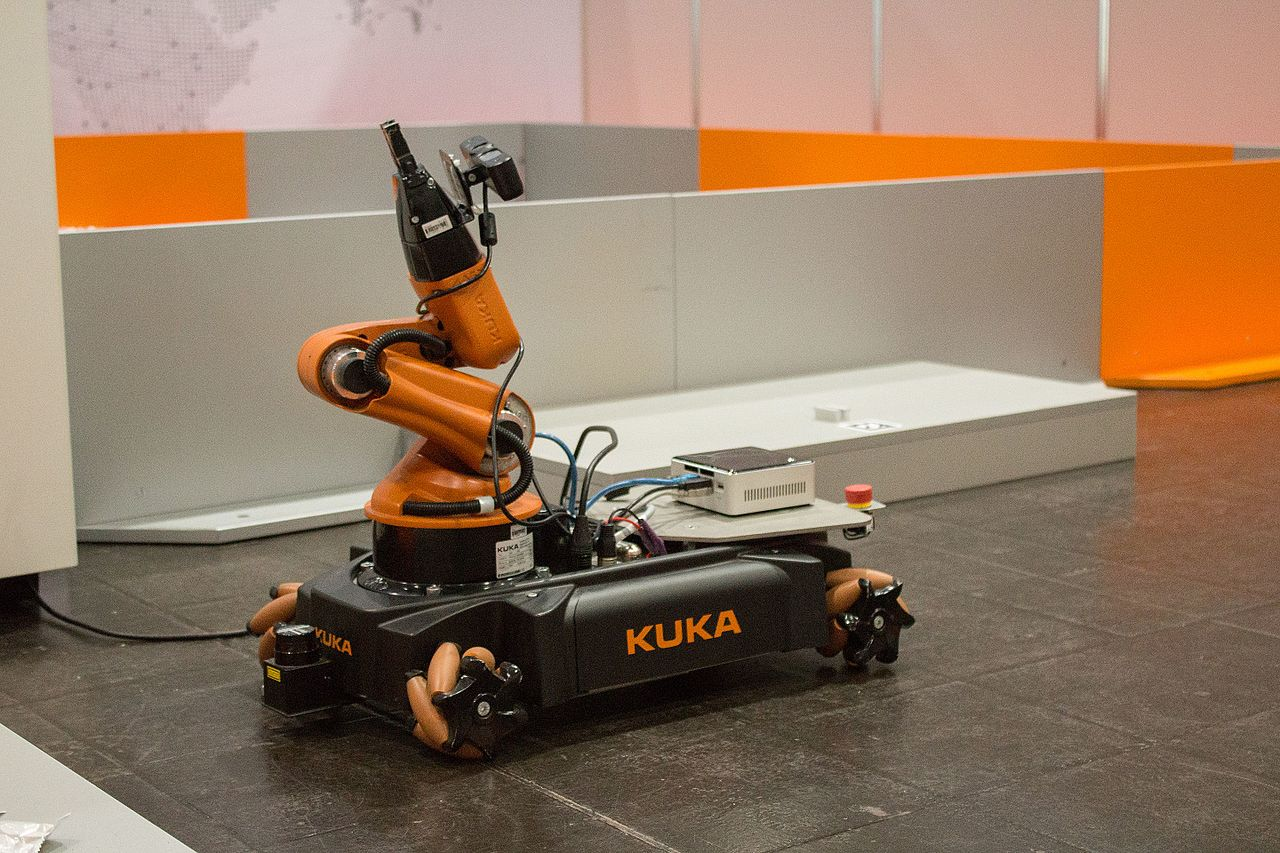
\includegraphics[width=\linewidth]{images/sec2/youbot_with_arm.png}
            \caption{The robot with the robotic arm attached. \notes{[cite]}}
        \end{subfigure}
        \hfill
        \begin{subfigure}[t]{0.49\linewidth}
            \centering
            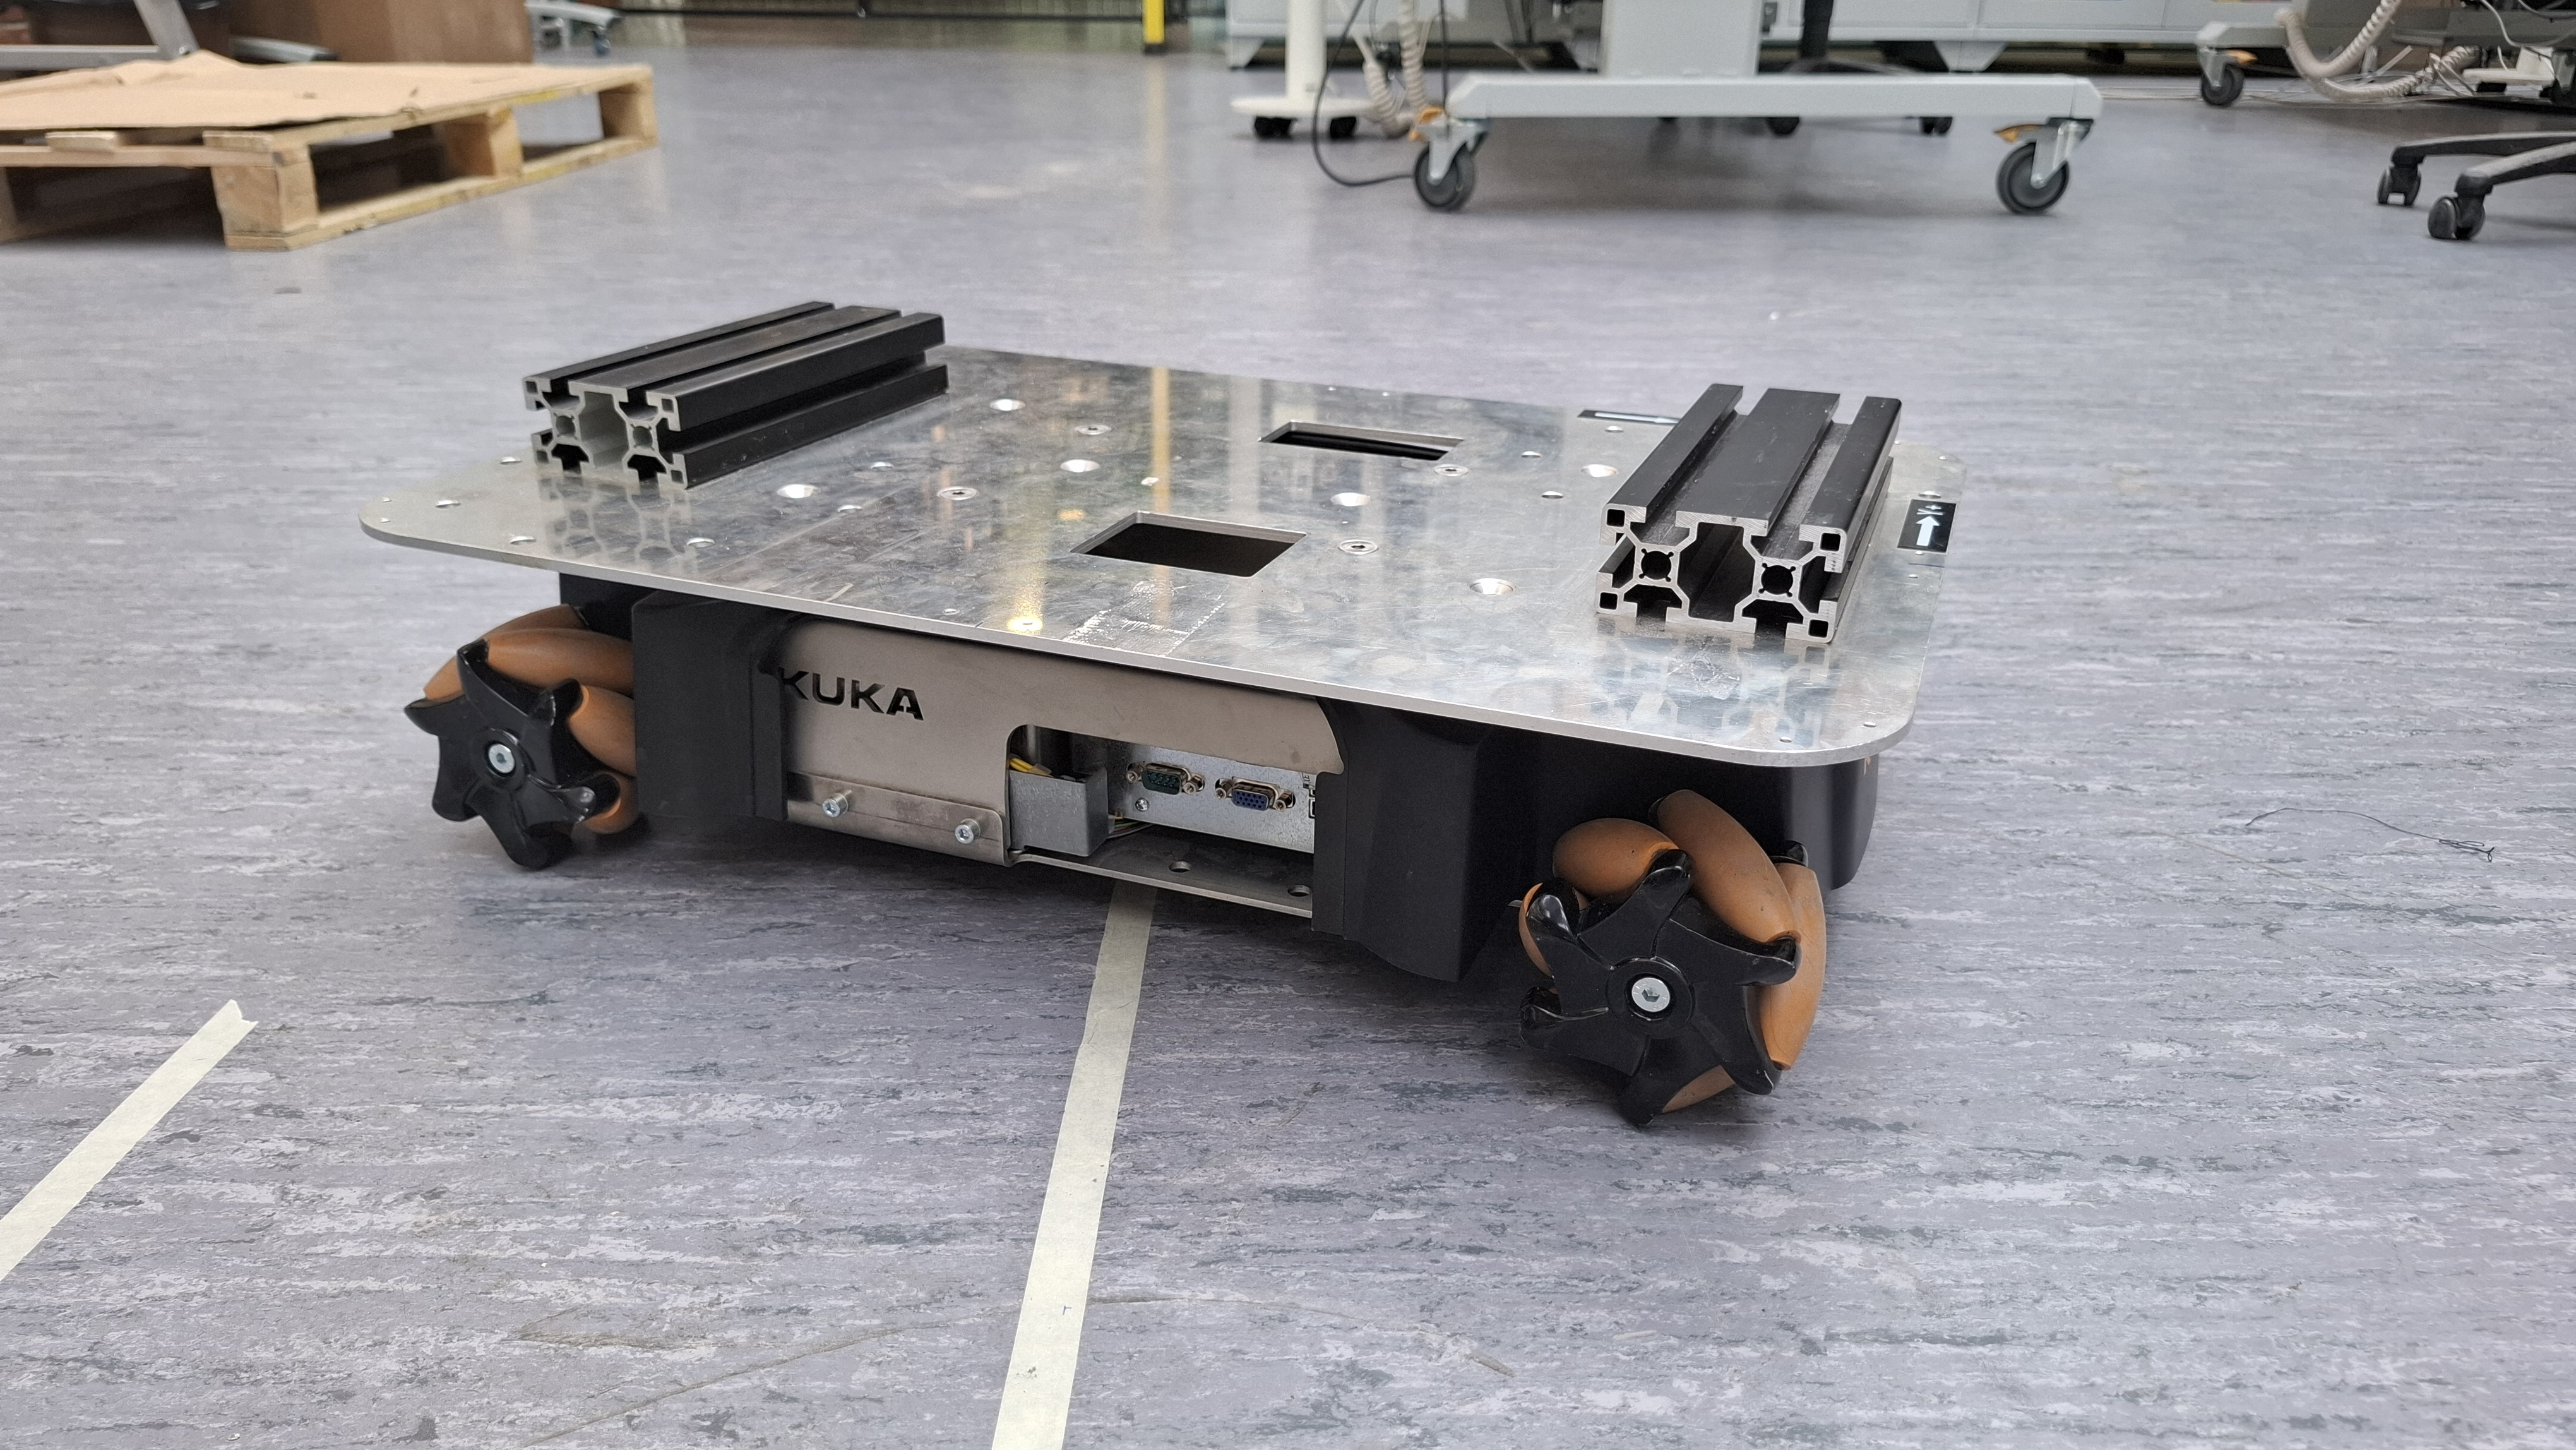
\includegraphics[width=\linewidth]{images/sec2/youbot_irl.jpg}
            \caption{The robot as used in the Aalto University Robotics Lab.}
        \end{subfigure}
        \caption{The YouBot.}
    \end{figure}

    \subsection{Onboard Computer}

    The onboard computer features a Intel Atom D510 @ 1.66GHz processor, with a 2GB DDR2 RAM and 32GB SSD hard drive. 

    The computer currently runs Ubuntu 12.04.5 LTS with ROS Hydro, which is a decade-old version of the operating system and the robot operating system. Given the age of the OS and ROS, compatibility with modern libraries and software is limited. Essential drivers and wrappers were also available to enable communication with the robot's motors and sensors. These could be accessed directly through C++ programs or through ROS packages. For the purposes of this project, we have elected to focus on the latter to allow for a seamless integration with the ROS ecosystem in the future, alongside a level of standardization and ease of use.

    \subsection{Connection Interfaces}

    To interface with the onboard PC, the YouBot features panels with several connection ports. The top panel of the robot contains two EtherCAT ports for consistent real-time communication with motion-oriented systems (i.e. robotic manipulators), and a standard Ethernet port for wired interfacing with an external computer or network. Adjacent to these communication ports are a power button and a small screen that displays input voltage and ON/OFF state of the onboard PC and motors (Figure~\ref{fig:youbot-screen}). Furthermore, the right side of the robot features a panel with a VGA port for video output, as well as six USB 2.0 ports for connecting peripherals such as a keyboard, mouse, or wireless adapter (Figure~\ref{fig:youbot-usb}). 

    \begin{figure}[H]
        \centering
        % Row 2
        \begin{subfigure}[t]{0.49\linewidth}
            \centering
            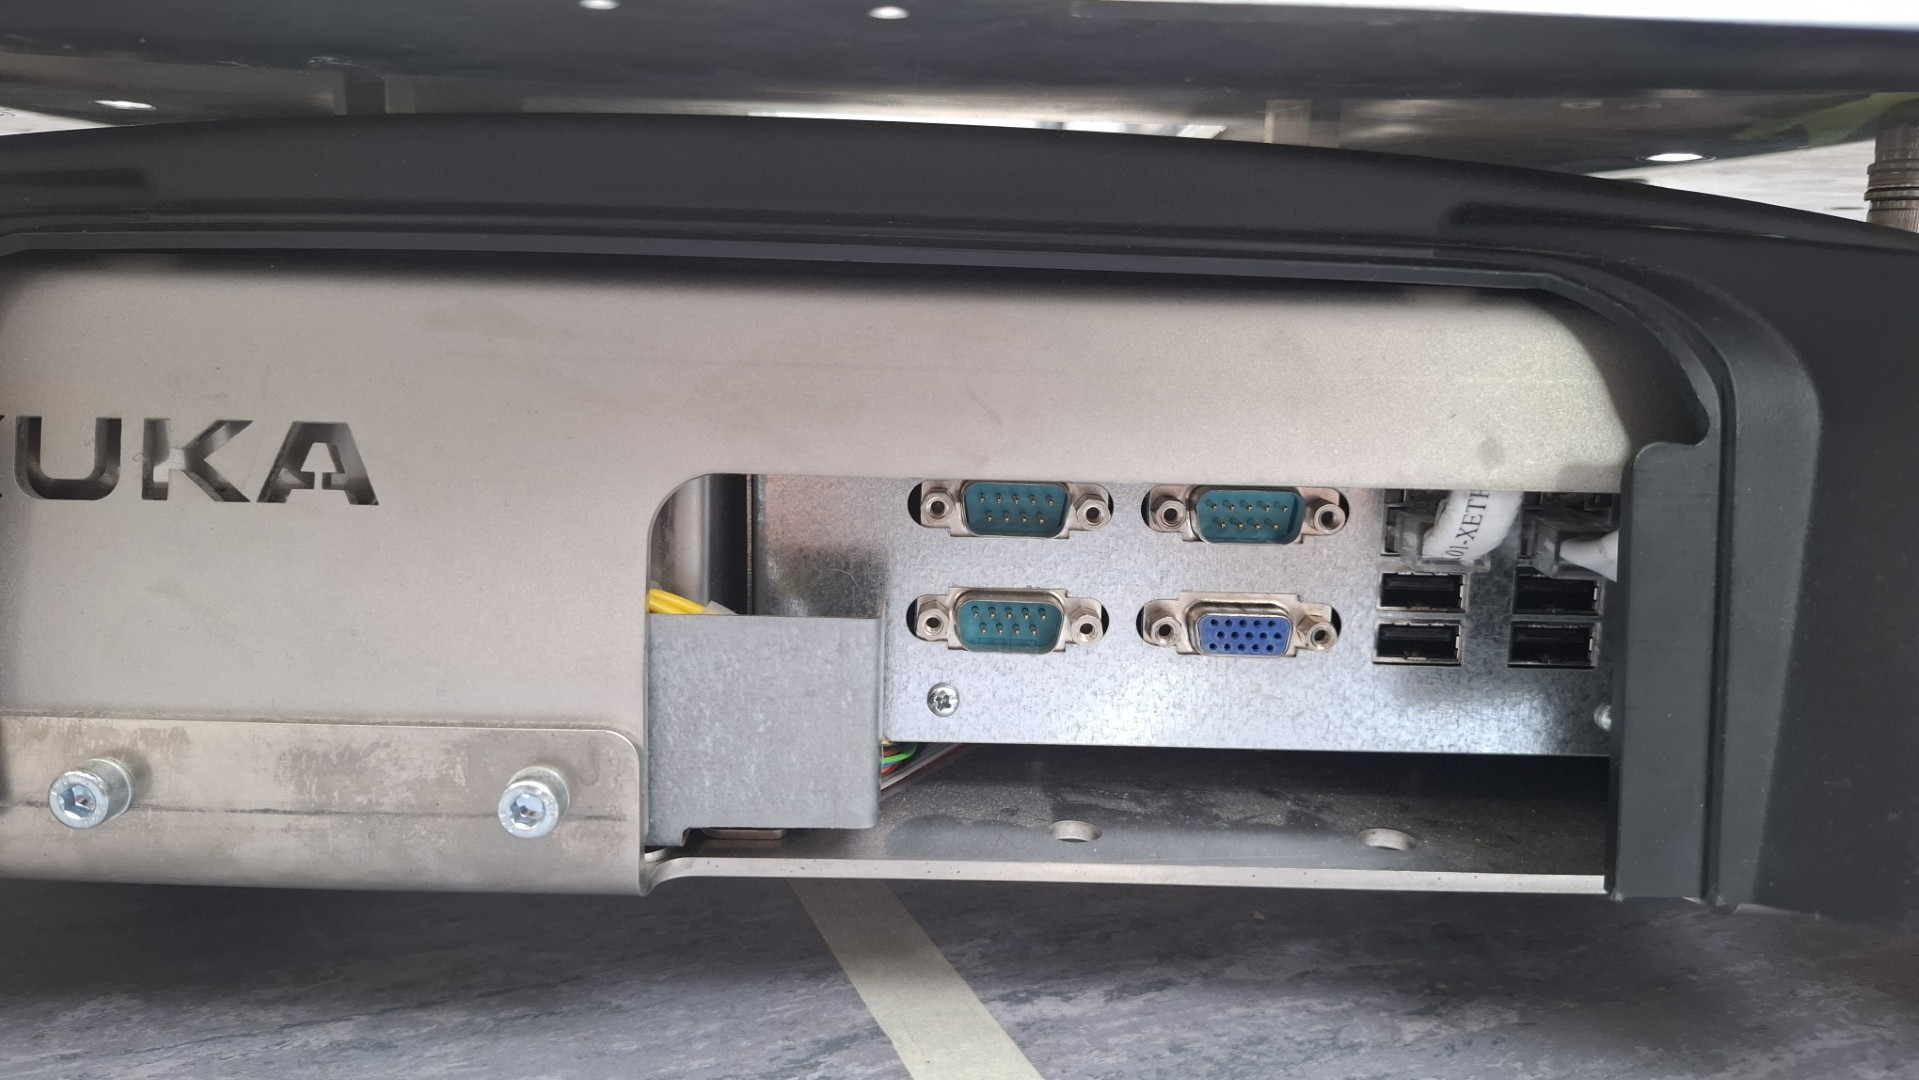
\includegraphics[width=\linewidth]{images/sec2/youbot_usb_ports.jpg}
            \caption{The right side of the robot, showing the VGA and USB ports.}
            \label{fig:youbot-usb}
        \end{subfigure}
        \hfill
        \begin{subfigure}[t]{0.49\linewidth}
            \centering
            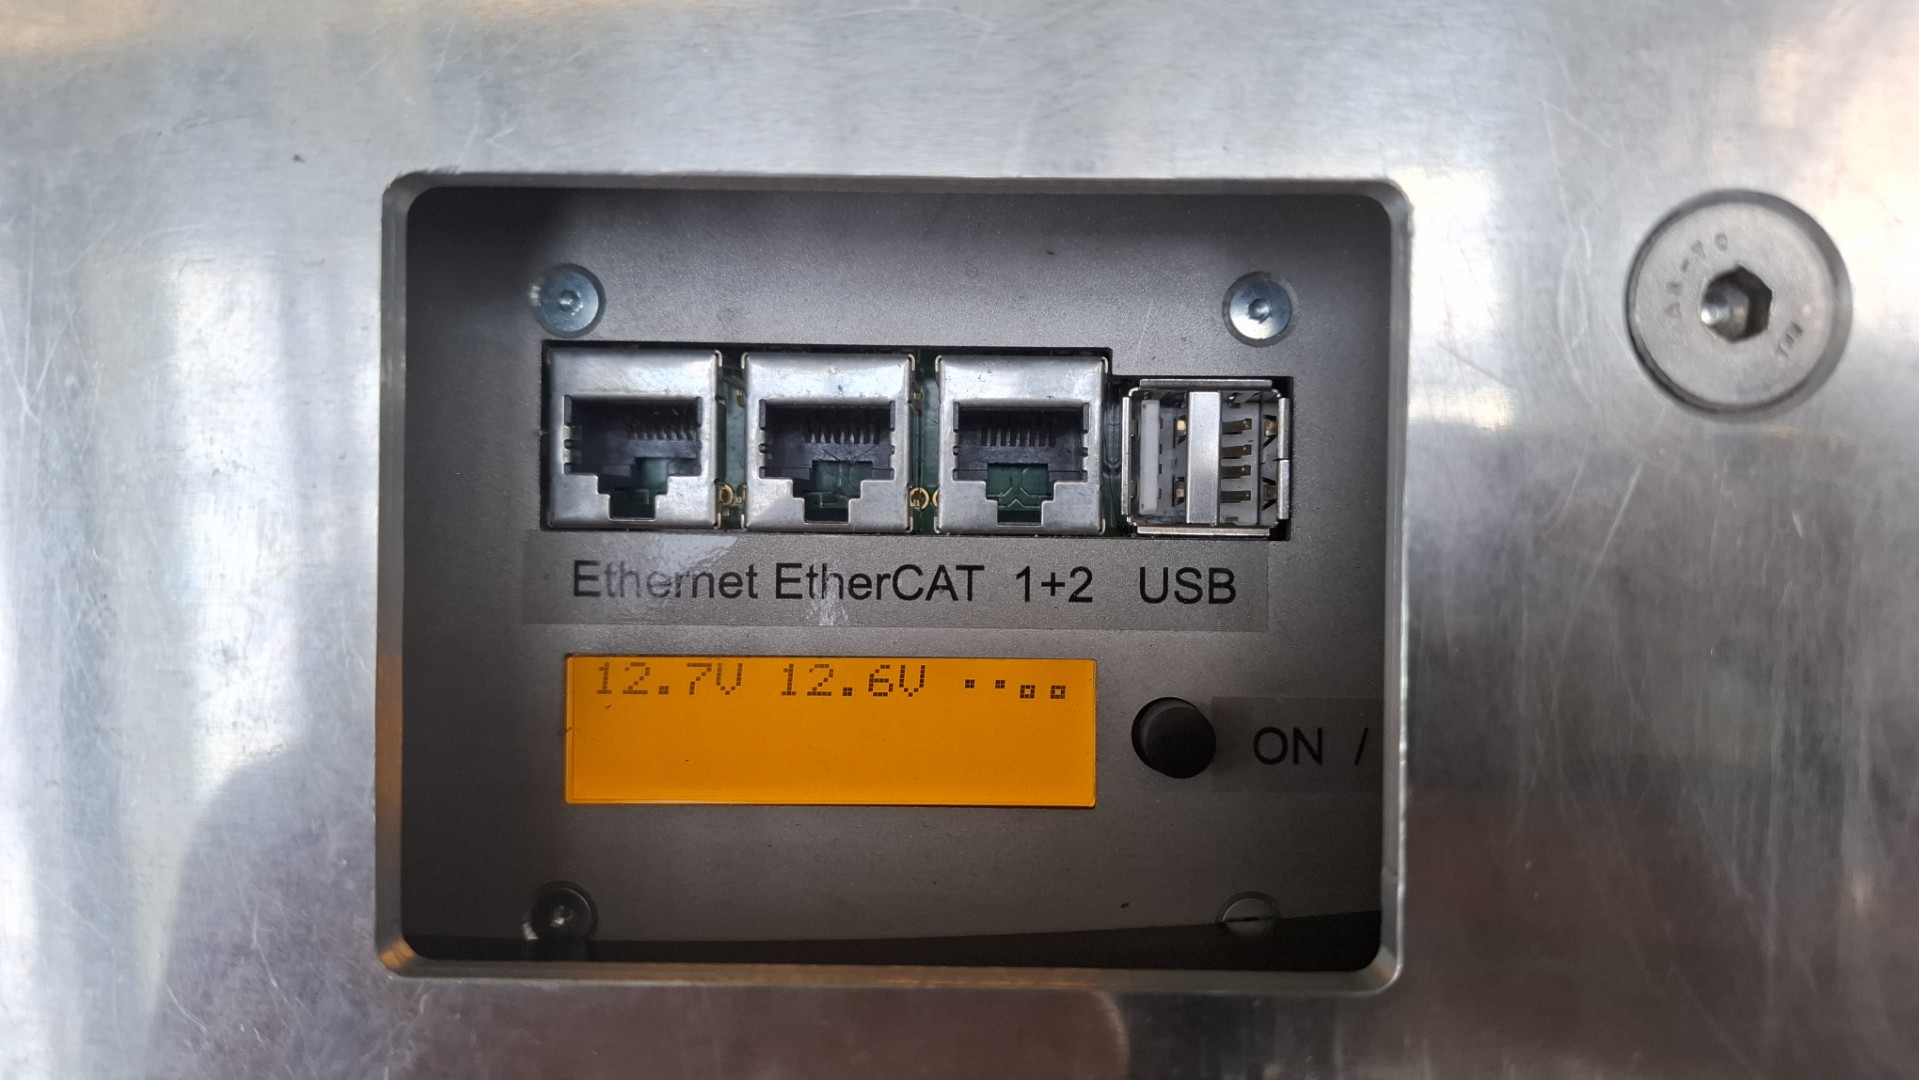
\includegraphics[width=\linewidth]{images/sec2/youbot_screen.jpg}
            \caption{The onboard computer screen, alongside the power button and EtherCAT/Ethernet ports.}
            \label{fig:youbot-screen}
        \end{subfigure}

        \caption{Connection points on the YouBot.}
        \label{fig:youbot-connections}
    \end{figure}


    \subsection{Power}

    The YouBot is powered by a 24V power supply, which can be connected through a 3-pin XLR connector located on the top panel of the robot. Additionally, the base includes two 24V 3-pin XLR output ports, which are intended for powering external components such as robotic manipulators or sensors (Figure~\ref{fig:youbot-power}).

    \begin{figure}[H]
        \centering
        \begin{subfigure}[t]{0.49\linewidth}
            \centering
            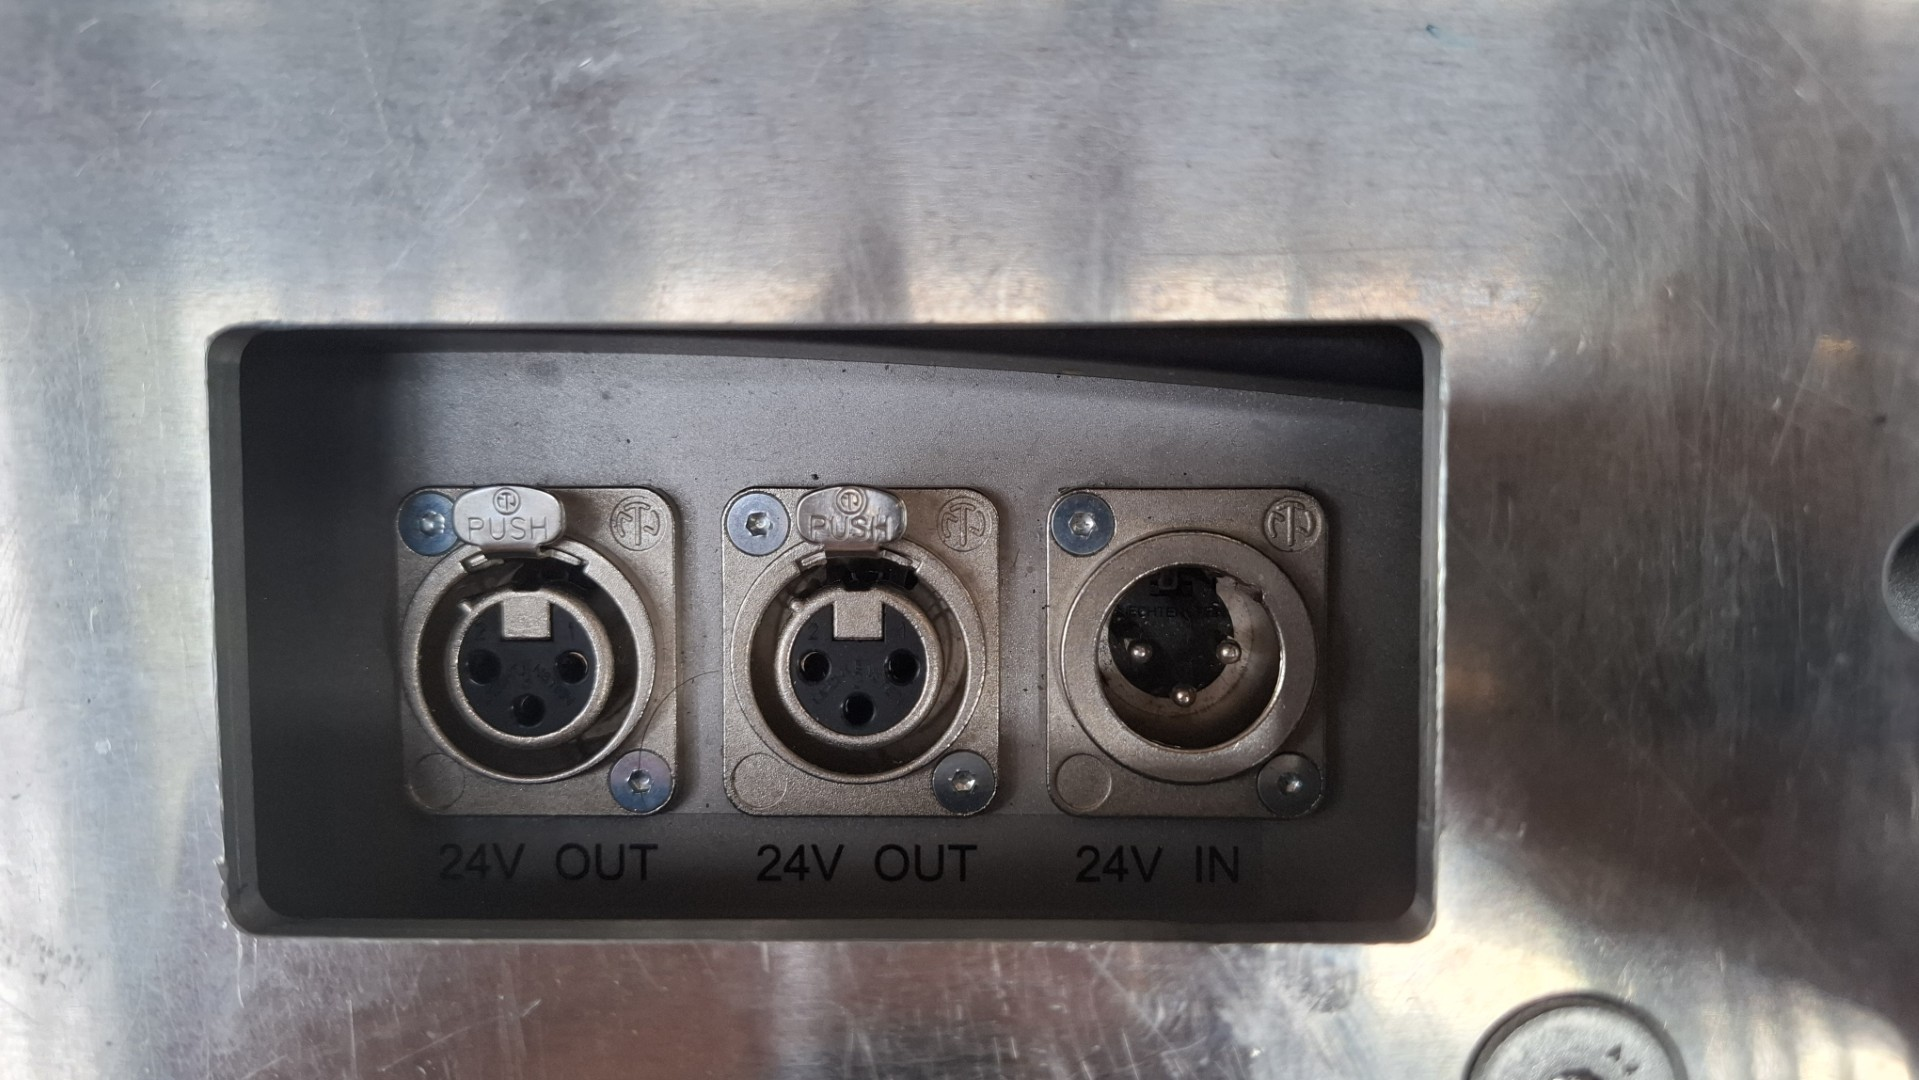
\includegraphics[width=\linewidth]{images/sec2/youbot_power.jpg}
            \caption{The power input and output ports.}
            \label{fig:youbot-power}
        \end{subfigure}
        \hfill
        \begin{subfigure}[t]{0.49\linewidth}
            \centering
            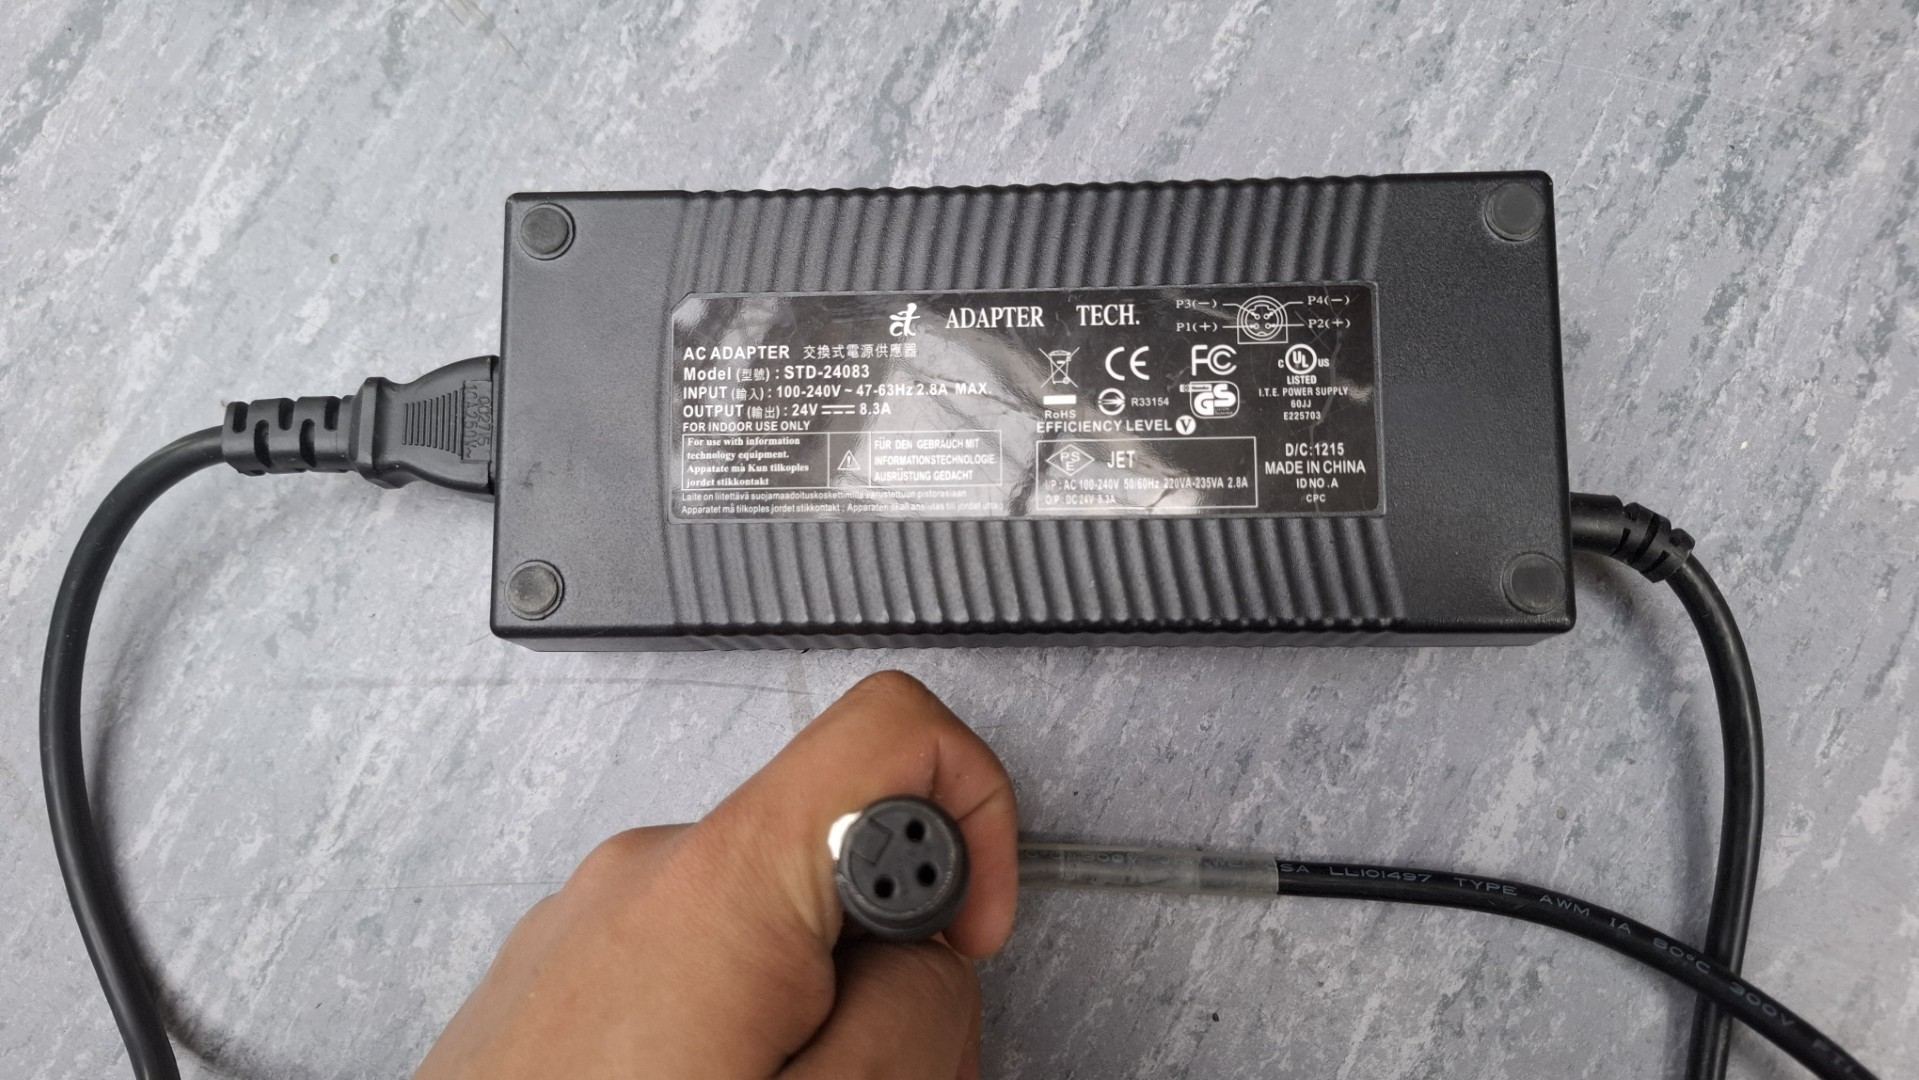
\includegraphics[width=\linewidth]{images/sec2/power_adapter.jpg}
            \caption{The 24V power adapter used to power the YouBot.}
        \end{subfigure}
        \caption{Power supply components for the YouBot.}
    \end{figure}

    However, continuously powering the YouBot through a wall connection is not ideal for the goal of mobile robotics. Thus, the YouBot was also originally equipped with a sealed lead-acid (SLA) battery (Figure~\ref{fig:youbot-battery}) . This battery had a capacity of 5Ah and provided an approximate runtime of 90 minutes. This battery furthermore connects to the robot via a 4-pin XLR connector, and is located in a dedicated slot on the left side of the robot (Figure~\ref{fig:youbot-battery-holder}). %While the 4-pin XLR connector is not standard for power supply (it is typically used for audio equipment), it is very robust and secure for the purposes of a mobile robot. This lead-acid battery is of dimensions 23cmx9.4cmx7.3cm.

    \begin{figure}[H]
        \centering
        \begin{subfigure}[t]{0.49\linewidth}
            \centering
            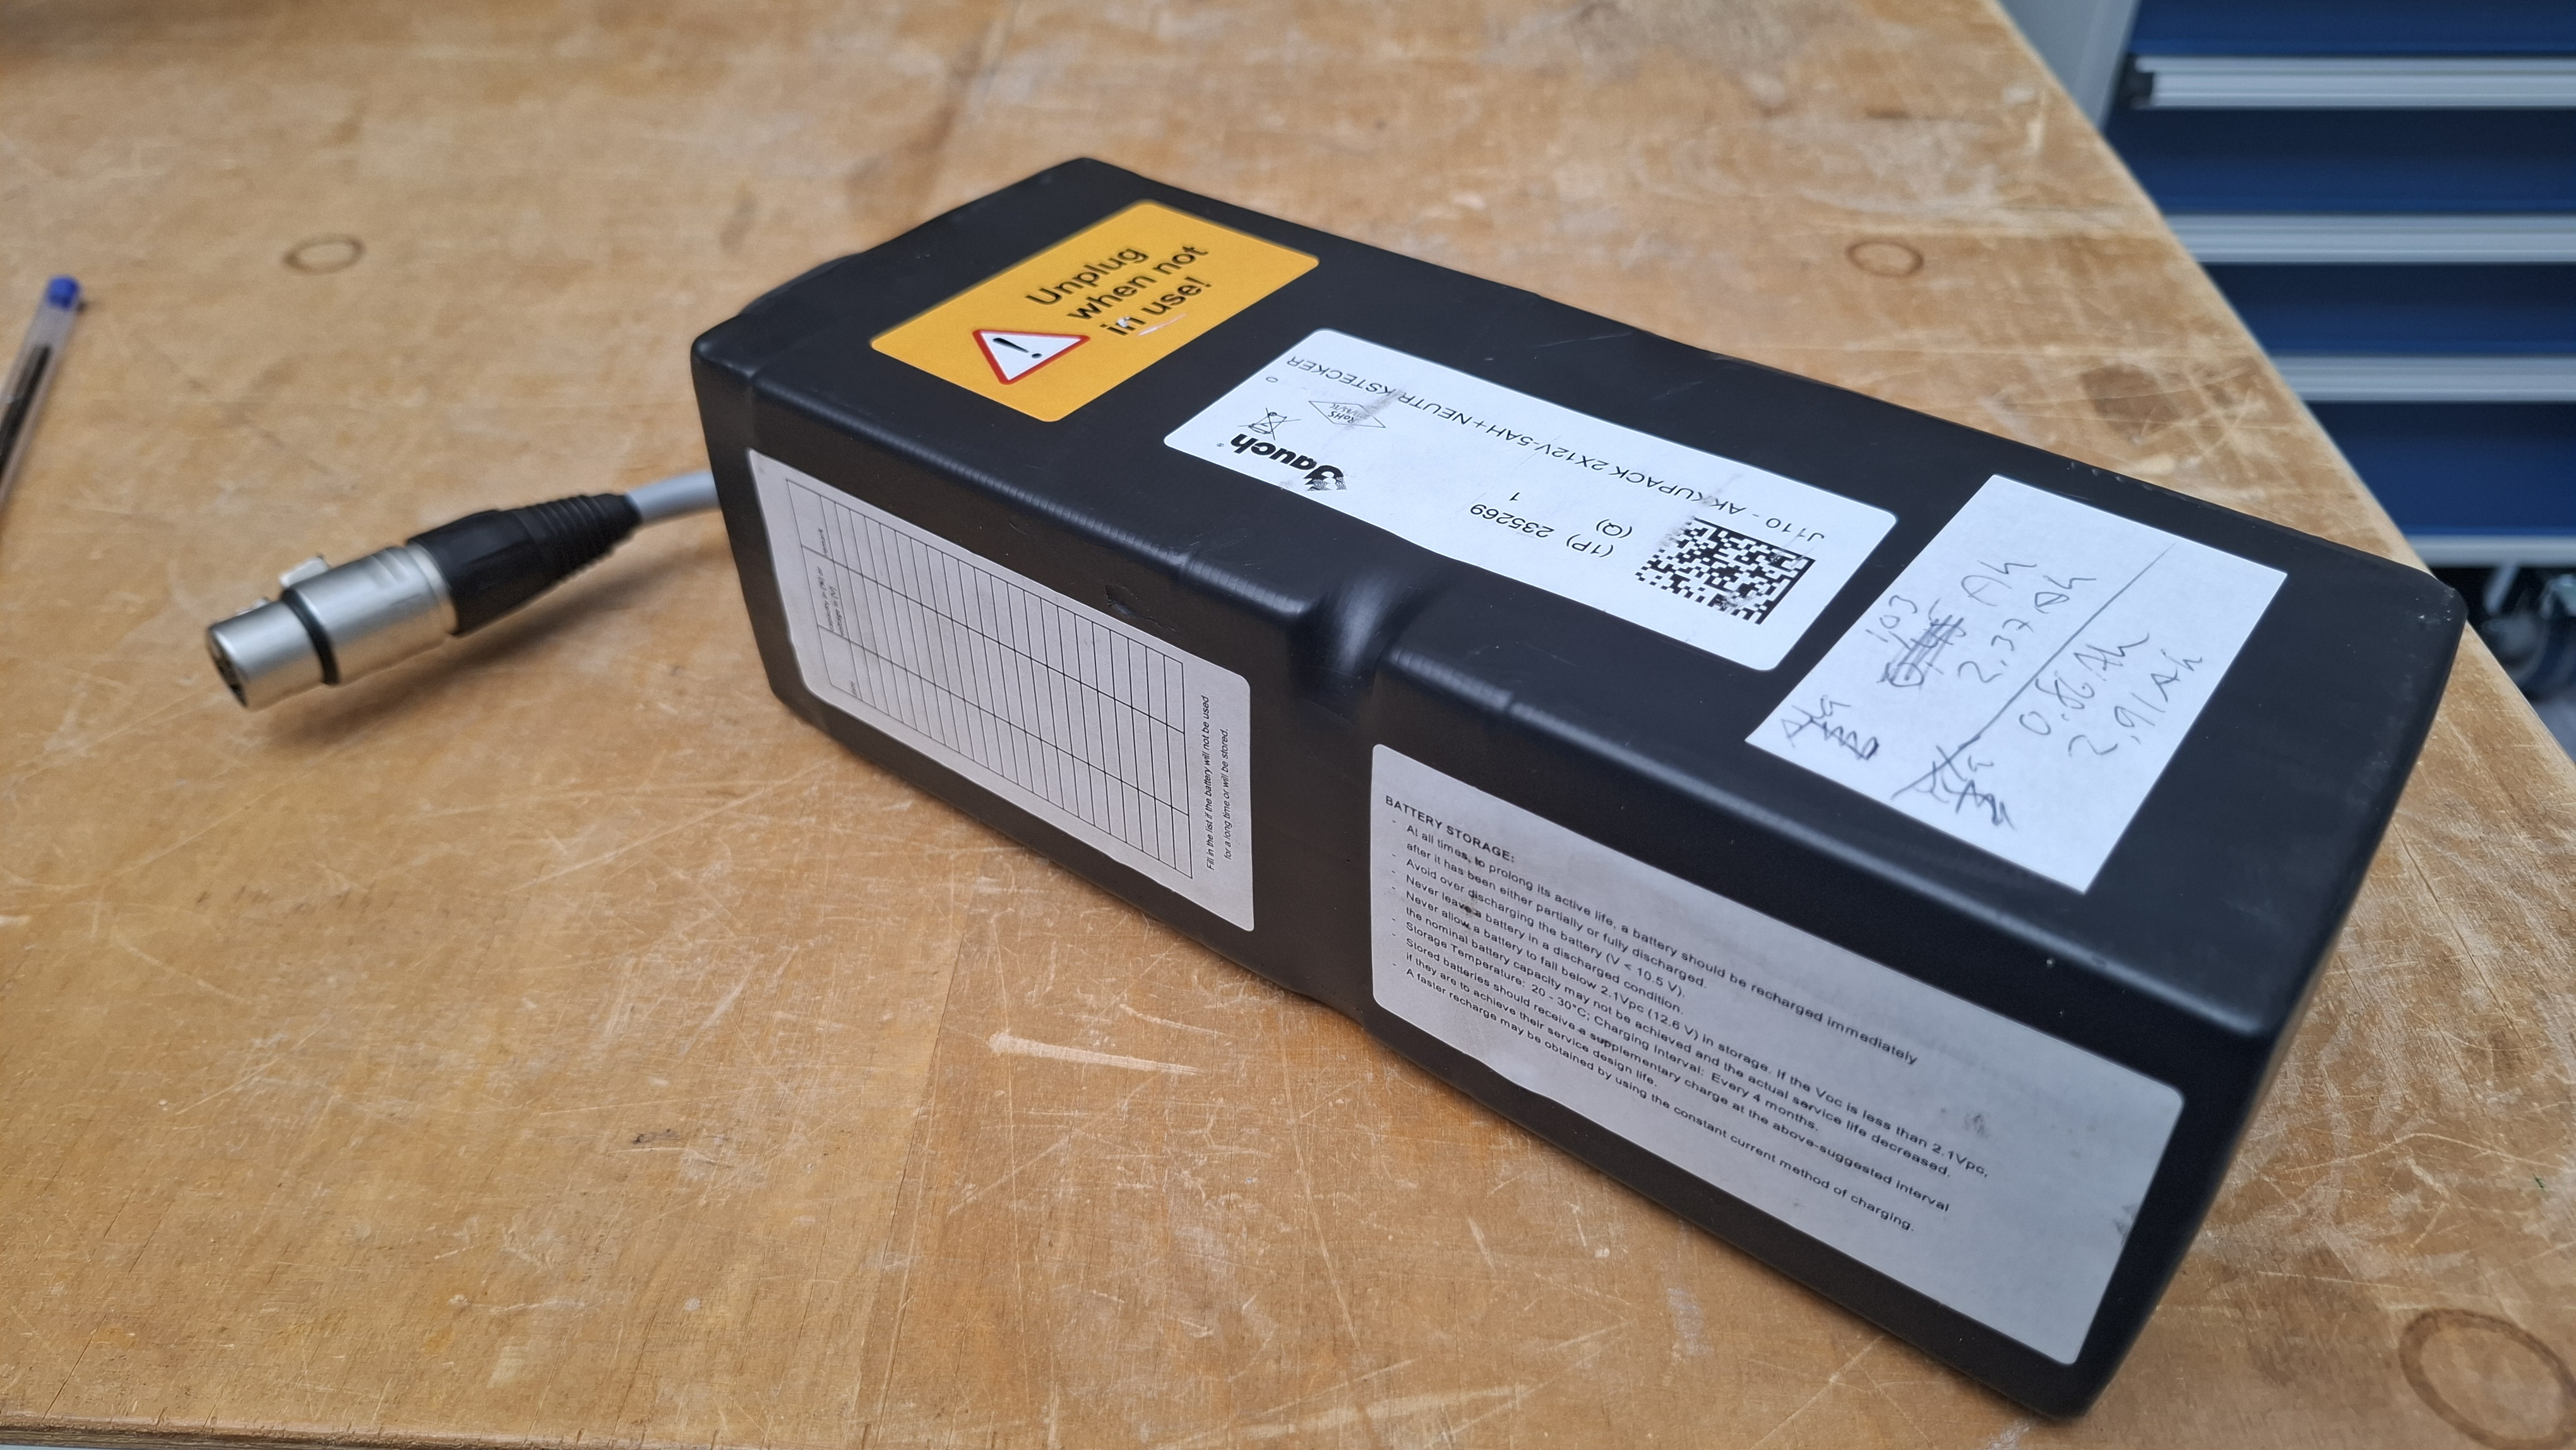
\includegraphics[width=\linewidth]{images/sec2/youbot_battery.jpg}
            \caption{The original SLA battery.}
            \label{fig:youbot-battery}
        \end{subfigure}
        \hfill
        \begin{subfigure}[t]{0.49\linewidth}
            \centering
            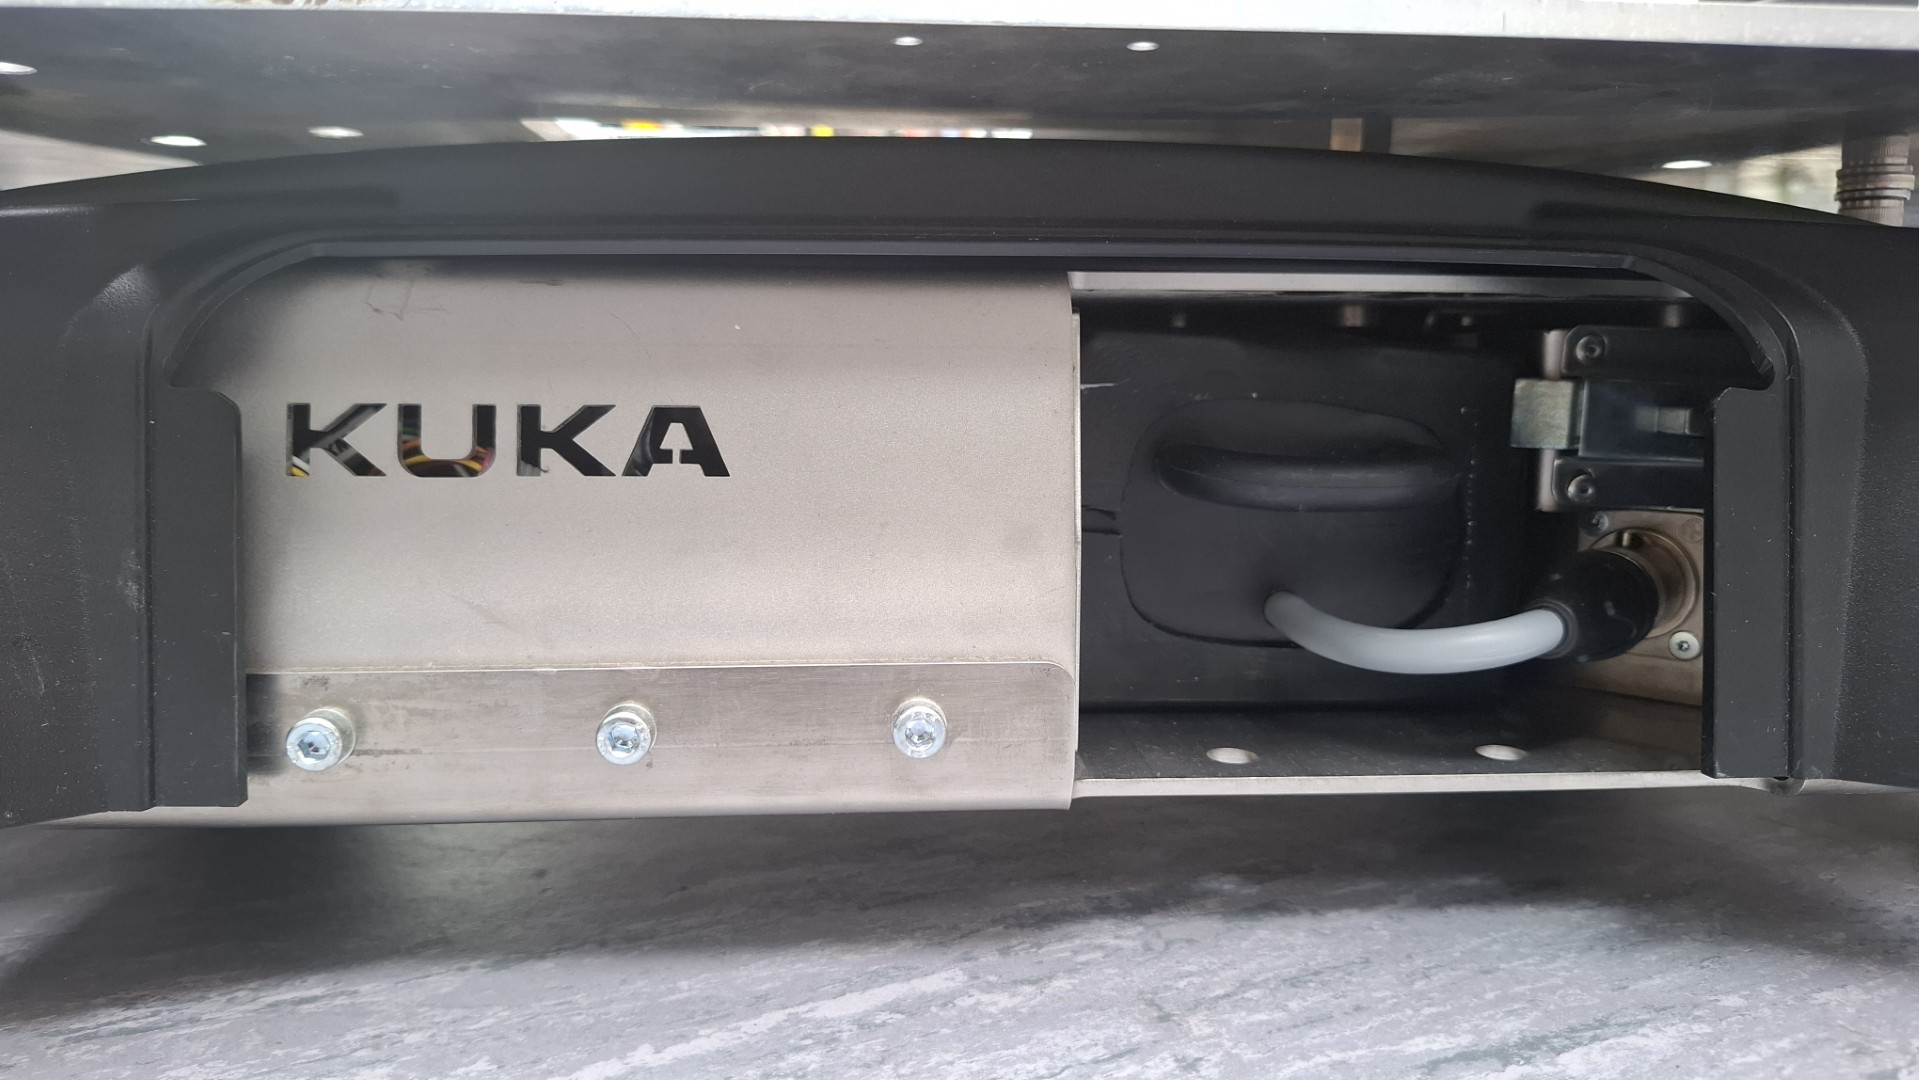
\includegraphics[width=\linewidth]{images/sec2/youbot_battery_holder.jpg}
            \caption{The left side of the robot, showing the battery in its holder.}
            \label{fig:youbot-battery-holder}
        \end{subfigure}
        \caption{Power supply connection points of the YouBot.}
    \end{figure}

    Upon receiving the robot, four SLA batteries were available: three of them were the original units supplied with the YouBot, and the fourth was a makeshift replacement assembled by the lab engineer, Vesa Korhonen, in 2019. Unfortunately, none of these batteries were functional. The original units had degraded beyond usability, and the makeshift battery had similarly deteriorated over time.

    As a result, the robot could not operate on battery power in its current state and required a constant wired connection to a wall outlet—an obvious limitation for a mobile robotics platform. A battery replacement would be ideal to restore the robot's potential mobility. 

    \subsection{Sensors}
    
    Alongside the robot base and various hardware components, the YouBot was also equipped with a variety of sensors to enhance perception and navigation. These included a Kinect v1 camera and two Hokuyo URG-04LX laser rangefinders. 

    \subsubsection{Kinect}  

    The Kinect v1 camera is a depth and RGB camera that was originally designed and sold in tandem with the XBOX 360 to support motion tracking and gaming. Due to its low cost, high availability and ease of use, it had indirectly become a popular choice in the robotics community for perception tasks. 

    Access to the Kinect's sensor data can be achieved through the use of open-source software such as libfreenect \notes{[cite]}. The retrieved data can then be processed using computer vision libraries such as OpenCV to enable the autonomous navigation as previously described. 

    \begin{figure}[ht]
        \centering
        %/flushleft
        %/flushright
        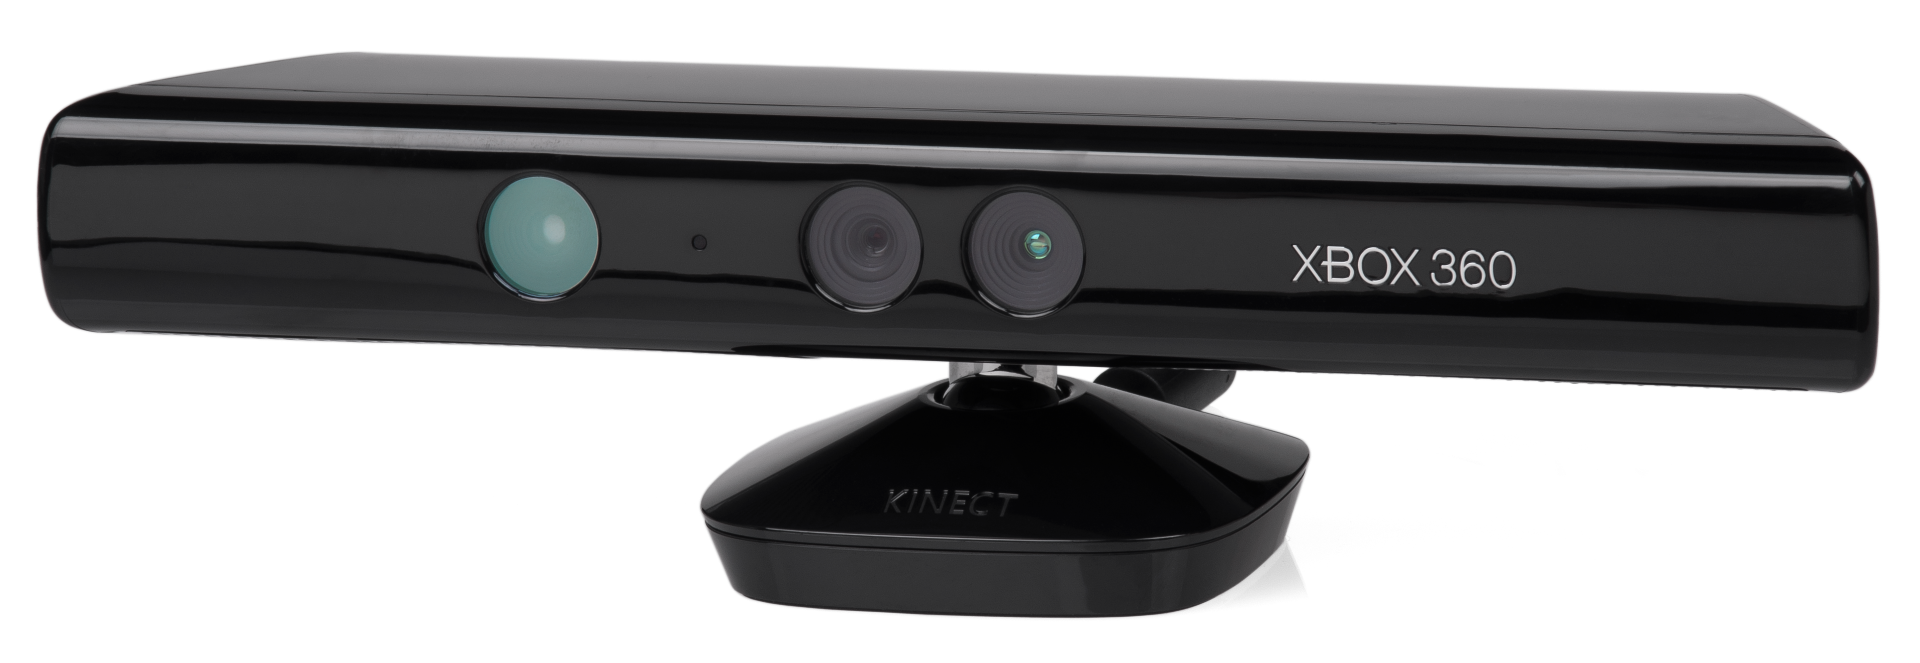
\includegraphics[width=0.5\linewidth]{images/sec2/kinectv1.png}
        \caption{The Kinect v1 camera module.}
    \end{figure}


    \subsubsection{Hokuyo URG-04LX Laser Rangefinder}

    The Hokuyo URG-04LX is a lightweight 2D laser rangefinder that is commonly used in robotics research. It provides high-resolution distance measurements in a 240-degree field of view and can detect objects upto 4 meters away with an accuracy of \(\pm10\) mm. It communicates with the onboard computer using a serial interface, enabling straightforward integration into existing systems for mapping, localization, and obstacle avoidance tasks. 

    \begin{figure}[ht]
        \centering
        %/flushleft
        %/flushright
        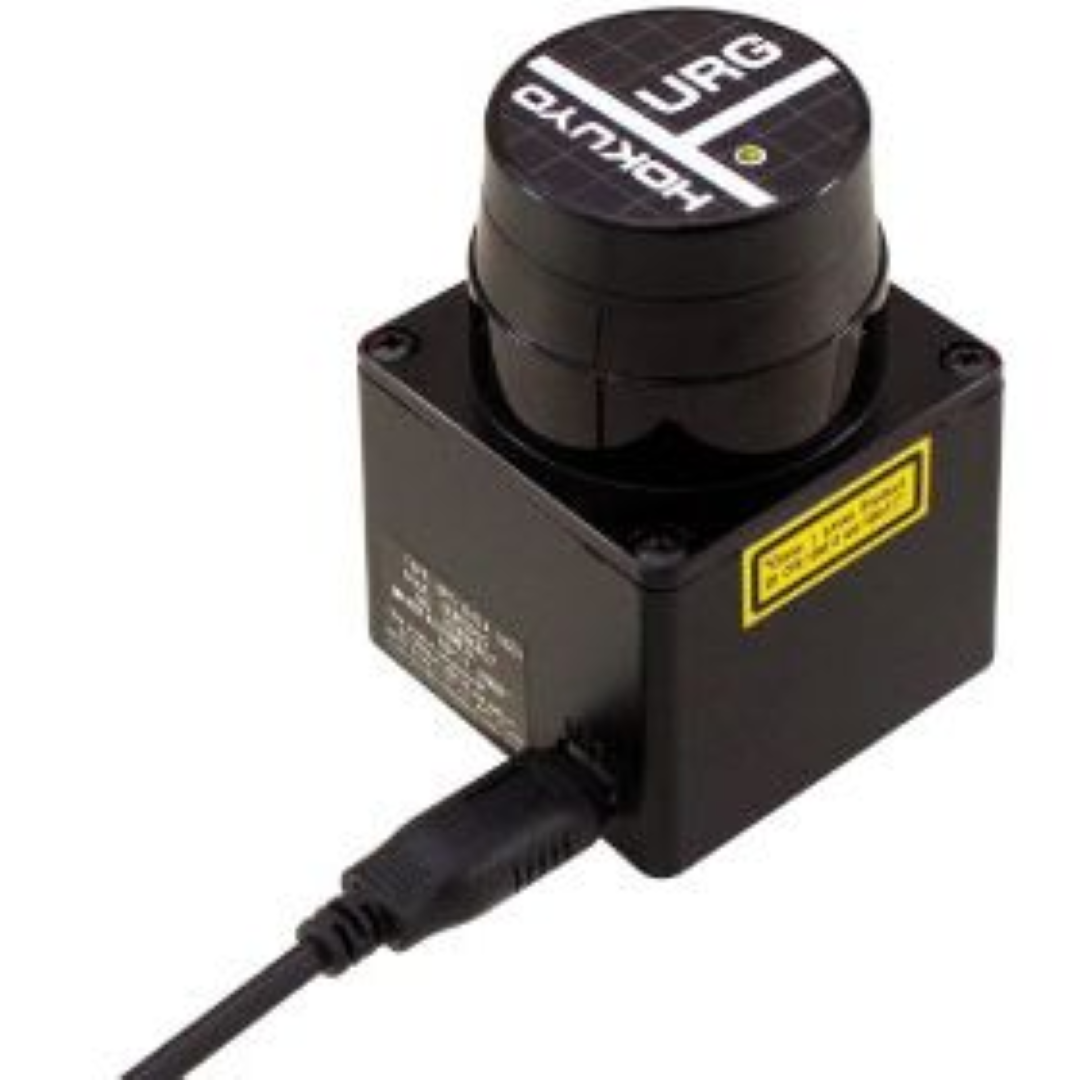
\includegraphics[width=0.25\linewidth]{images/sec2/hokuyo.png}
        \caption{The Hokuyo URG-04LX laser rangefinder.}
    \end{figure}

    \subsection{Additional Hardware Components}

    
    \notes{DESCRIBE THE INITIAL INSPECTION IN FULL HERE! TALK ABOUT THE PILLAR STUFF AND NUTS AND WHATNOT AS WELL!!!!}

    The YouBot also came with a variety of additional components and accessories to assist with sensor mounting and operation. These included a variety of nuts, bolts, and screws, as well as a hex key and several horizonal and vertical pillars. These pillars can be combined in a variety of ways to create a stable and secure mounting platform for the sensors. 

    The attached top panel is a sensor and mounting plate, designed to allow for the convenient attachment of various sensors and accessories. [cite https://web.archive.org/web/20160613151621/http://www.youbot-store.com/accessories/mounting-and-sensor-plate]

    
    \begin{figure}[H]
        \centering
        \begin{subfigure}[t]{0.49\linewidth}
            \centering
            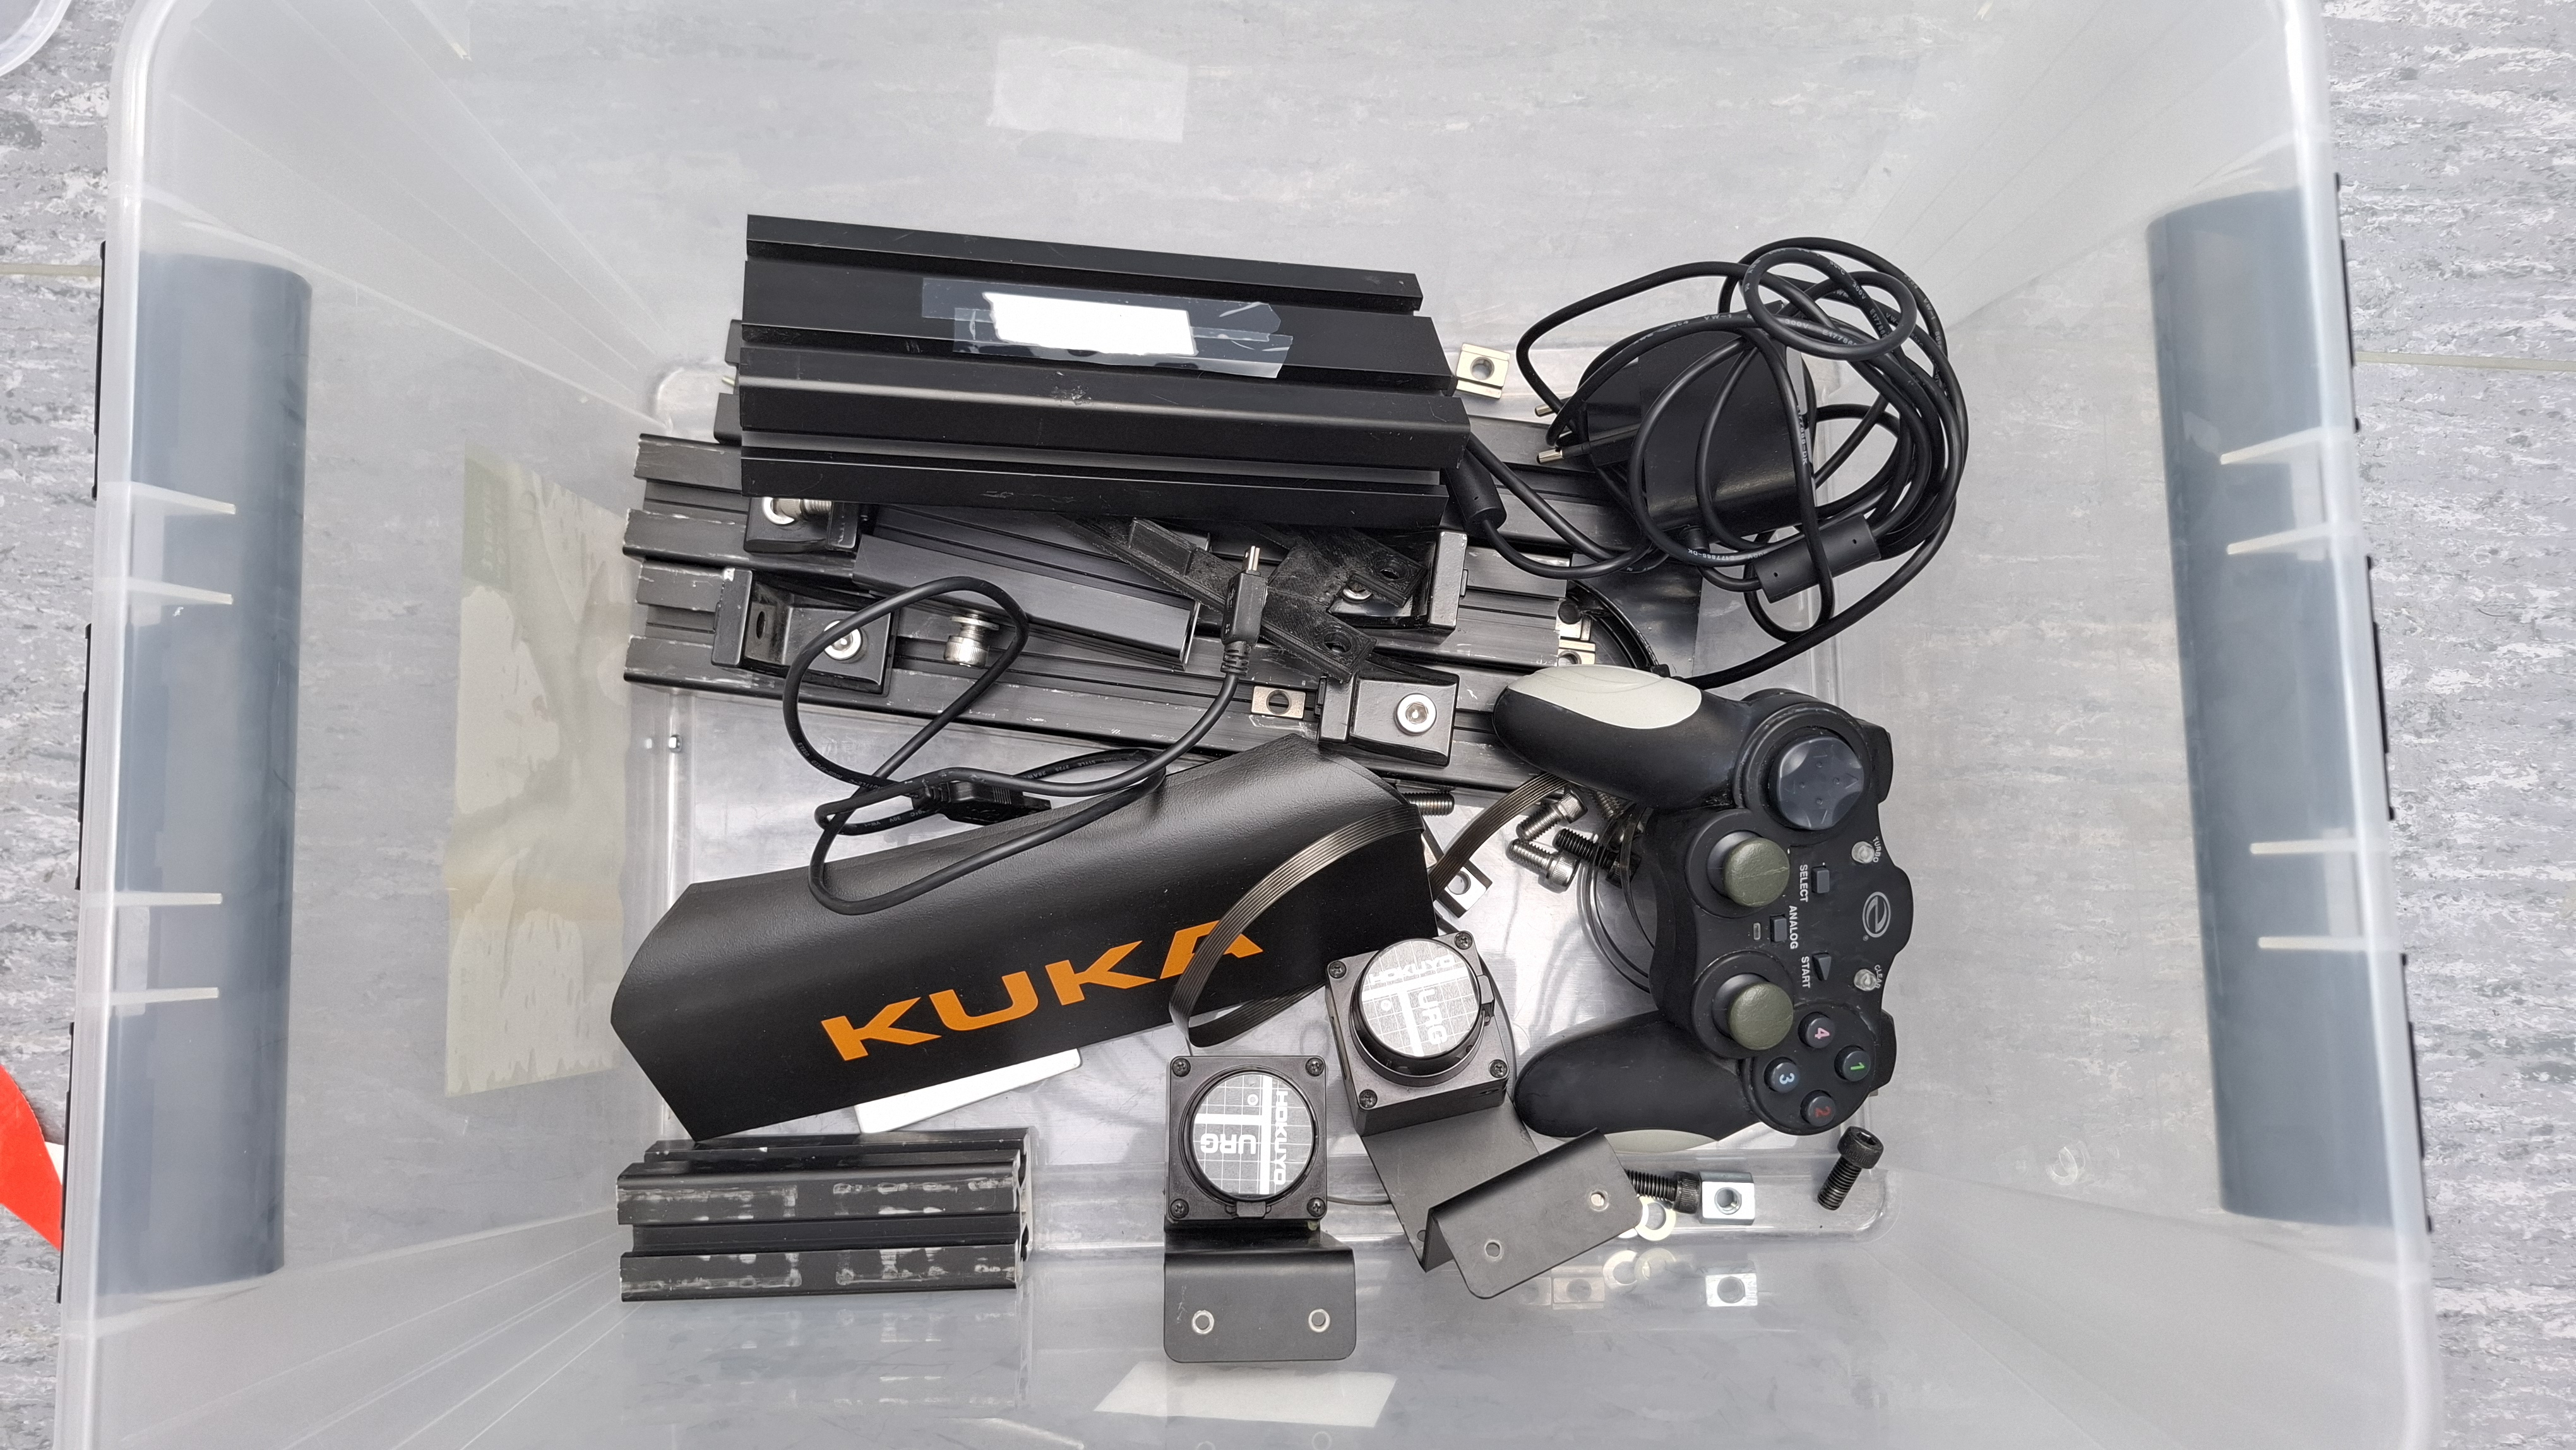
\includegraphics[width=\linewidth]{images/sec2/box2.jpg}
            \caption{Various pillars, nuts and bolts amongst other components.}
        \end{subfigure}
        \hfill
        \begin{subfigure}[t]{0.49\linewidth}
            \centering
            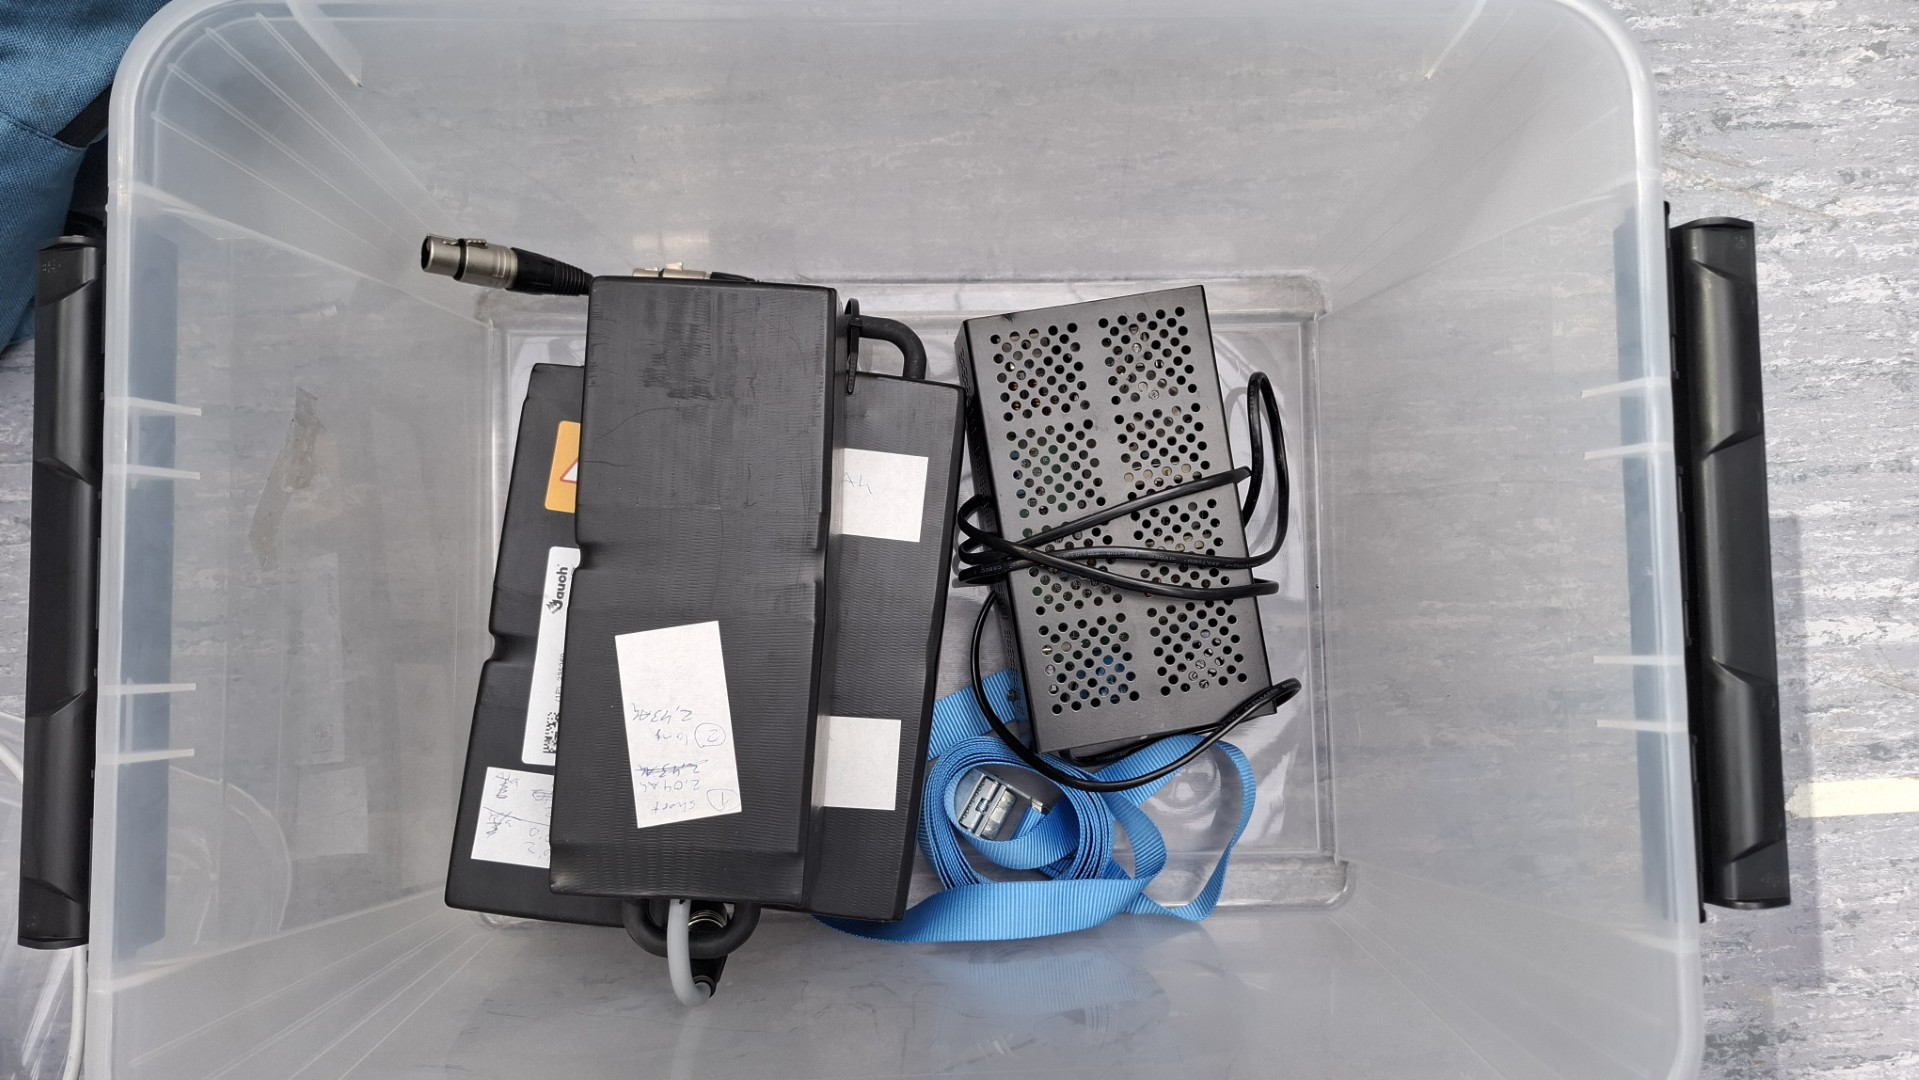
\includegraphics[width=\linewidth]{images/sec2/box1.jpg}
            \caption{The box containing previously used batteries and miscellaneous components.}
        \end{subfigure}
        \caption{Additional hardware components supplemented with the YouBot.}
    \end{figure}

    \subsection{Documentation}

    The documentation for the KUKA YouBot is sparse and unavailable for the most part. KUKA has removed most references to the product from their website, and the original youbot-store.com website is no longer available. Furthermore, the only available user manual for the YouBot online is a decade-old PDF file that was uploaded by a third-party user, and is marked as a draft version from 2013. 

    Thankfully, the YouBot was marketed as an open-source platform, and the drivers as well as various parts of software are available on GitHub. Furthermore, we were able to find some more information about the YouBot through the Wayback Machine, which had archived parts of the original website. While this archive is not complete by any means and is very tedious to comb through, it provides us with a powerful tool to piece together data about the YouBot and its use cases during its hayday.

    We've also taken the liberty of citing some YouBot related projects here.

    \notes{add images of some of the more interesting websites here, and some of the images regarding the youbot's statistics.}
    \subsection{Initial Project Goals}

    Considering the hardware and software components of the YouBot, the initial goals of this project involved a comprehensive revival of the robot and the enabling of autonomous navigation using the Kinect camera. This would showcase the potential of the YouBot in cutting-edge research despite its age. 

    Teach \& Repeat (T\&R) was considered to be an ideal candidate to allow for the autonomous navigation. This\notes{[cite]} is a two-phase robotic navigation method where a robot is first "taught" a path via human guidance or pre-recoded data. The sensor data captured during this phase can then be used to allow the robot to autonomously "repeat" the path later on, even in different environments.

    T\&R only requires a single camera for a basic implementation. It is a relatively simple method to implement through the use of open-source software and libraries, such as OpenCV and ROS. Furthermore, it is robust to changes in the environment and can dynamically correct errors through the use of visual odometry. As such, it has been a very popular research topic within the field of robotics, particularly in the context of mobile robots \notes{[cite]}. Much of the work done on extending T\&R aims to improve this robustness and scalability for a variety of sensors and use-cases. 

    \adi{I'm not sure how the ROS stack would look like, or if its necessary to explain. Discuss with advisor}
    \begin{figure}[ht]
        \centering
        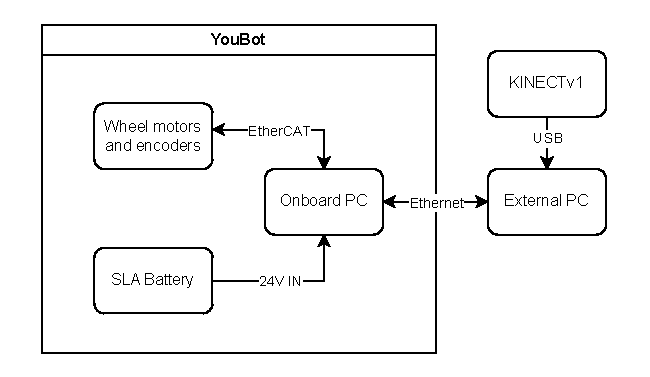
\includegraphics[width=\linewidth]{diagrams/sample.pdf}
        \caption{System Diagram}
        \label{fig:system-diagram}
    \end{figure}


    Here, figure [] shows an example of how the architecture for this system would have been implemented. This would have involved a wired connection to an external computer running ROS2 Jazzy and directly connected to the Kinect camera mounted on top of the YouBot. The onboard computer would have been used to control the motors and communicate with the sensors, while the external computer would have handled the processing and navigation tasks. The onboard computer and external computer would commuicate through a ROS1-ROS2 bridge, allowing for seamless integration of the two systems. 

    However, considering the age of the YouBot, lack of personal knowledge regarding robotics, as well as incompatible software, it was realised that this was not feasible. We will be discussing our new goals in the next section. 

    \pagebreak
    
    \section{Project Overview}

    \subsection{Technical Goals}

    The technical goals for this project involve the deployment and quantification of the robot's capabilities, particularly in terms of navigation and odometry. This would involve the following goals: 
    \begin{itemize}[noitemsep, topsep=0pt]
        \item Inspecting the initial physical state of the YouBot
        \item Enabling the robot start up
        \item Enabling the running of the original demos
        \item Enabling the running of the ROS interface
        \item Enabling the ROS1-ROS2 bridge
        \item Enabling wireless connections to external computers using SSH and Ethernet
        \item Writing custom programs to control the YouBot
        \item Testing the movement and odometry of the YouBot
        \item Measuring the quality of movement and odometry by measuring their error
        \item Replacing the current deprecated batteries with a usable battery
        \item Documenting the revival process and potential future applications of the YouBot
    \end{itemize}
    
    The set of goals that have been formulated have deviated from the original goals, which were formulated based on experimenting and identifying the limitations of the robot. 

    \subsection{Learning Objectives}

    The learning objectives for this project involve the following:
    \begin{itemize}[noitemsep, topsep=0pt]
        \item Develop hands-on experience in restoring and operating a legacy robot platform (KUKA YouBot)
        \item Gain proficiency in Linux systems and environment setup for robotics development
        \item Learn to write and use Bash scripts to automate setup, build, and deployment workflows
        \item Understand the architecture of the Robot Operating System (ROS1 \& ROS2), and learn to configure and launch ROS-based systems
        \item Learn to establish and manage secure communication with robotic systems using SSH and Ethernet
        \item Write and deploy custom ROS nodes for basic motion control of the YouBot platform
        \item Understand the principles of robot navigation and odometry, including error measurement and correction techniques
        \item Learn methods for documenting system restoration, experimental results, and identifying directions for future development
    \end{itemize}

    \subsection{System Architecture}
    Our intended setup was to use the YouBot as a mobile base with the Kinect camera mounted on top of it. The onboard computer of the YouBot would only be used to control the motors and communicate with the sensors. The actual bulk of the processing would be done on a seperate computer that runs ROS2 and enables the necessary navigation and perception stacks.
    
    \begin{figure}[H]
        \centering
        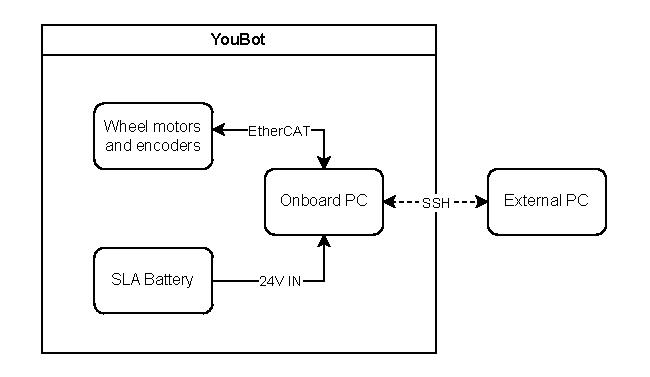
\includegraphics[width=\linewidth]{diagrams/new_arch.drawio.pdf}
        \caption{New System Diagram}
        \label{fig:new-system-diagram}
    \end{figure}

    \pagebreak

    \section{System Development}
    \subsection{Booting up the YouBot}

    The initial inspection was carried out as described in section 2. Since the onboard battery was completely dead, I connected the YouBot to the 24V power supply and booted it up. On long pressing the power button, the screen flashed on and I could see the voltage input for the robot, alongside options to turn the PC and motors on/off seperately. 

    After connecting a monitor using VGA and keyboard and mouse using USB, I was able to boot up the onboard PC and use it as any other computer. The wireless adapter connected to this onboard computer was also functional, and was able to connect to the internet. This meant one could theoretically SSH into the onboard computer from a personal laptop, but I was unable to do so at that time due to a lack of a static IP address.
    
    I was able to see the following software installed on the onboard computer: insert ROS version here and discuss the github repos that were already installed here. 

    The installed software includes youbot\_driver, which provides the necessary drivers to communicate with the robot's motors and sensors. Additionally, a complete ROS stacks were installed (youbot-ros-pkg) to provide ROS support for the YouBot. Alternatively, interfacing can be done with the simpler youbot\_driver\_ros\_interface package, which provides a minimal set of ROS nodes to control the YouBot. The latter has been used for the purposes of this project to simplify the interaction with the robot. Additionally, youbot\_description provides the necessary URDF files to describe the robot's kinematics and dynamics, allowing for simulation and visualization in RViz and Gazebo. Finally, youbot\_applications provides a set of example applications and demos to get started with the YouBot. There are additional open-source from the official youbot GitHub account that can be seen from here.  

    
    \notes{insert pictures showing failed stuff}
    \subsection{Initial Configuration}

    The ROS interface as well as the relevant demo programs were attempted to be run. The C++ demo programs were unable to detect any devices on the eth0 port, which was not the port the motors were using. The ROS interface was also unable to ping itself and start \code{roscore}. This was due to the onboard computer not being bind to the correct static IP address, which is necessary for the ROS interface to function properly.

    Furthermore, the onboard computer did not have a static IP address, which meant that it could not be accessed through Ethernet. These three issues were thus configured and fixed.

    \subsubsection{ROS Networking Configuration (.bashrc)}
    The ROS networking configuration was set up by editing the \code{.bashrc} file on the onboard computer. This file is used to configure the environment variables for the ROS interface, and is executed every time a new terminal is opened. The following lines were added to the \code{.bashrc} file:

    \begin{lstlisting}[style=plain]
    export DSD_IP=localhost

    # April 2025 : DSD Final Project settings
    export ROS_IPV6=off
    export ROS_HOSTNAME=$DSD_IP
    export ROS_MASTER_URI=http://$DSD_IP:11311
    export ROS_IP=$DSD_IP

    export ROS_PACKAGE_PATH=$ROS_PACKAGE_PATH://home/youbot/youbot_driver:/home/youbot/ros_stacks:/home/youbot/applications
    export LIBGL_ALWAYS_SOFTWARE=1

    source /opt/ros/hydro/setup.bash
    source ~/DSD/devel/setup.bash #this will be covered later.
    \end{lstlisting}

    This will set the ROS networking configuration to use the local host as the IP address, and will ensure that the ROS interface can communicate with itself. The \code{ROS_PACKAGE_PATH} variable is also set to include the necessary directories for the YouBot drivers and applications. To test whether ROS is now able to communicate with itself, the following command was run:
    \begin{lstlisting}[style=plain]
$   roscore 
    \end{lstlisting}
    If the command runs successfully, it means that the ROS interface is now able to communicate with itself and is ready to be used. 

    \subsubsection{Ethernet Configuration (/etc/network/interfaces)}    
    
    To fix the ethernet issue, \code{ifconfig} was ran to check the current network interfaces and their IP addresses. The output showed that \code{eth0} was not configured with a static IP address, and was instead using DHCP.

    This was rectified by adding a static IP address for \code{eth0} to the \code{/etc/network/interfaces} file. This file is used to configure the network interfaces on the onboard computer as needed. The file was opened and the following lines added:

    
    \begin{lstlisting}[style=plain]
    auto eth0
    iface eth0 inet static
        address 192.168.10.1 # The IP address used by the YouBot
        netmask 255.255.255.0
    \end{lstlisting}
    
    After saving the file, the network interface was restarted using the following command:

    \begin{lstlisting}[style=plain]
$   sudo /etc/init.d/networking restart
    \end{lstlisting}

    Initially, the following commands were used to set the static IP address: 
    \begin{lstlisting}[style=plain]
$   sudo ip addr add 192.168.1.200/24 dev eth0
    \end{lstlisting}
    however, this would automatically delete itself inconsistently due to the Network Manager. This was thus changed to the above method, which would set the static IP address permanently. This is much more convenient long term. 

    One can then connect another computer to the YouBot using an Ethernet cable and set its static IP address to another address in the same subnet, such as \code{192.168.10.2}. Test the connection by pinging the YouBot's IP address from the other computer:
    \begin{lstlisting}[style=plain]
$   ping 192.168.10.1
    \end{lstlisting}
    If the ping is successful, the connection is established and the YouBot can be accessed through a wired connection. One can also use SSH to connect to the YouBot from another computer using the following command:
    \begin{lstlisting}[style=plain]
$   ssh youbot@192.168.10.1
    \end{lstlisting}
    where \code{youbot} is the default username of the onboard computer. The default password is \code{youbot}.

    \subsubsection{Youbot Driver Configuration (~/youbot\_driver/config/youbot-ethercat.cfg)}

    The YouBot driver configuration file was also edited to change the port from \code{eth0} to \code{eth1}. This was done by opening the file \code{~/youbot\_driver/config/youbot-ethercat.cfg} and changing the line:
    \begin{lstlisting}[style=plain]
    #EtherCAT port
    [EtherCAT]
    EthernetDevice = eth0
    \end{lstlisting}

    This will enable the YouBot driver to communicate with the motors and sensors through the correct port for the C++ demos. After saving the file, the YouBot driver can be started using the following command:
    \pagebreak

    \subsection{Running original demos}

    An attempt was made to run the original demos upon turning on the computer. These original demos are stored at \code{~/applications} locally (available on the YouBot's GitHub repository as \code{youbot_applications}). The demos are written in C++ and provide a simple interface to control the YouBot's motors and sensors. This includes a Hello World application to test the communication with the motors, as well as a keyboard control demo to enable primitive keyboard control.

    
    After the EtherCAT interfacing issue was fixed, one can run the original demos by going to the relevant directory and running the application. Remember to turn the motors on beforehand. 
    \begin{lstlisting}[style=plain]
$   cd ~/applications/hello_world_demo/bin
$   sudo ./youBot_HelloWorldDemo
    \end{lstlisting}
    \notes{add the feedback from the demo here}
    
    The output should show that the YouBot is able to communicate with the motors and sensors, and that the Hello World application is running successfully, by moving in the four cardinal directions.

    Additionally, the keyboard control demo can be run by going to the relevant directory and running the application. This will allow you to control the YouBot's movement using the keyboard. The following command can be used to run the keyboard control demo:
    \begin{lstlisting}[style=plain]
$   cd ~/applications/keyboard_control_demo/bin
$   sudo ./youBot_KeyboardControlDemo
    \end{lstlisting}
    \notes{add the feedback from the demo here}

    This shows that the YouBot is able to communicate with the motors and sensors as expected. However, running the original demos is very cumbersome and cannot be extended into a more complex system. As such, we will be using the ROS interface, as discussed in the next section. 

    \pagebreak

    \subsection{Running ROS Interface}

    After verifying that the original C++ demos functioned correctly, the focus was shifted towards using the ROS interface, which provides a more scalable and modular framework for robotics development. The ROS interface allows for the integration of higher-level capabilities such as visualization, mapping, planning, and logging.

    \subsubsection{Finding Installed Packages}
    Additionally, the following command was used to list installed packages:

    \begin{lstlisting}[style=plain]
$   rospack list
    \end{lstlisting}

    Among the key packages found were:

    \begin{itemize}
        \item \code{youbot_driver_ros_interface} – The core package providing ROS interfaces to the hardware.
        \item \code{youbot_teleop} – A keyboard teleoperation node.
        \item \code{youbot_common} – Shared definitions and URDF files.
        \item \code{youbot_description} – The robot model used for visualization and simulation.
    \end{itemize}

    \subsubsection{Launching the ROS Interface}

    The ROS environment was initialized as described earlier by sourcing the appropriate setup scripts in the \code{.bashrc} file. Once that was configured, the interface could be launched with:

    \begin{lstlisting}[style=plain]
$   roscore
$   roslaunch youbot_driver_ros_interface youbot_driver.launch
    \end{lstlisting}

    The driver was successfully able to connect to the hardware via EtherCAT and expose the motors and sensors to ROS.

    \subsubsection{Inspecting ROS Nodes and Topics}

    With the ROS system running, the following commands were used to inspect the active components:

    \begin{lstlisting}[style=plain]
$   rosnode list
$   rostopic list
    \end{lstlisting}

    Sample output from \code{rosnode list} included:

    \begin{itemize}
        \item \code{/youbot_driver} – The main node managing low-level hardware.
        \item \code{/rosout} – Standard logging node.
    \end{itemize}

    Sample topics included:

    \begin{itemize}
        \item \code{/joint_states} – Published joint positions and velocities.
        \item \code{/tf} – Coordinate transforms used for kinematics and visualization.
        \item \code{/cmd_vel} – Subscribed to for base velocity commands.
    \end{itemize}

    \subsubsection{Visualization with \code{rqt} and \code{rviz}}

    To visually inspect the robot’s state and perform debugging, both \code{rqt} and \code{rviz} were used.

    \begin{itemize}
        \item \code{rqt_graph} provided a real-time view of the node and topic communication.
        \item \code{rviz} allowed visualization of the robot’s URDF model, TF tree, joint states, and more.
    \end{itemize}

    \begin{lstlisting}[style=plain]
    $ rosrun rqt_graph rqt_graph
    $ rosrun rviz rviz
    \end{lstlisting}

    \pagebreak
    \subsection{ROS1-ROS2 Bridge}

    One of the first tasks I decided to embark on after getting the robot up and running was to set up the ROS1-ROS2 bridge. This was the most important link within the system, as it would allow the robot to seamless access the ROS2 navigation stack and enable it to access the computational resources of a more recent computer. However, the version of ROS1 on the robot is Hydro, which is more than a decade old and predates ROS2 development, i.e. it is not compatible with a ROS1-ROS2 bridge. 

    There are thus a handful of options to consider: One would be to upgrade the ROS1 version of the robot to a version that supports the bridge, such as Melodic or Noetic. However, this would require a significant amount of work and may cause compatibility issues with the outdated software on the robot. Another option would be to use a different computer with a more recent version of ROS1 and use it as a middleware between the robot and the ROS2 navigation stack. This would allow for a more seamless integration of the two systems, but would require additional hardware and software setup and create an unneccesarily complex system. 

    \pagebreak

    \subsection{Writing Custom Programs}

    Using the ROS demo packages as a reference, I was able to write my own custom programs to control the YouBot. This involved using the ROS packages and drivers on the onboard computer to send velocity commands to the motors through the \code{/cmd_vel} topic. While primitive, this provides a simple and intuitive way to control the robot's movement using Python scripts. This can be further extended to support autonomous navigation, sensor feedback, or integration with external systems.

    \subsubsection{Creating a Catkin Workspace}

    Before writing custom ROS programs, a \code{catkin} workspace must be created. This workspace will contain all custom packages and nodes. The following commands create a basic workspace:

    \notes{write code for creating a catkin workspace here.}

    \begin{lstlisting}[style=plain]
    $ mkdir -p ~/DSD/catkin_ws/src
    $ cd ~/DSD/catkin_ws/
    $ catkin_make
    \end{lstlisting}

    After building the workspace, it must be sourced to update the ROS environment:

    \begin{lstlisting}[style=plain]
    $ source devel/setup.bash
    \end{lstlisting}

    It is recommended to add this line to the \code{.bashrc} file so that it is sourced automatically in every new terminal:

    \begin{lstlisting}[style=plain]
    echo "source ~/DSD/catkin_ws/devel/setup.bash" >> ~/.bashrc
    \end{lstlisting}

    \subsubsection{Creating a Custom Package}

    Once the workspace is initialized, a new package can be created within the \code{src} directory:

    \begin{lstlisting}[style=plain]
    $ cd ~/DSD/catkin_ws/src
    $ catkin_create_pkg youbot_control rospy std_msgs geometry_msgs
    $ cd ~/DSD/catkin_ws
    $ catkin_make
    \end{lstlisting}

    This creates a new package named \code{youbot\_control} with dependencies on the necessary ROS message types.

    \subsubsection{Writing a Python Control Script}

    Inside the package, a Python script can be written to publish velocity commands to the robot. For example:

    \begin{lstlisting}[style=plain]
    $ cd ~/DSD/catkin_ws/src/youbot_control
    $ mkdir scripts
    $ touch scripts/simple_move.py
    $ chmod +x scripts/simple_move.py
    \end{lstlisting}

    Sample content for \code{simple_move.py}:

    \begin{lstlisting}[style=plain]
    #!/usr/bin/env python

    import rospy
    from geometry_msgs.msg import Twist

    rospy.init_node('simple_move')
    pub = rospy.Publisher('/cmd_vel', Twist, queue_size=10)

    move_cmd = Twist()
    move_cmd.linear.x = 0.1  # Move forward at 0.1 m/s
    move_cmd.angular.z = 0.0

    rate = rospy.Rate(10)  # 10 Hz
    for _ in range(50):  # Publish for 5 seconds
        pub.publish(move_cmd)
        rate.sleep()

    # Stop
    move_cmd.linear.x = 0.0
    pub.publish(move_cmd)
    \end{lstlisting}

    This script sends a simple forward command to the robot for 5 seconds and then stops.

    To run the script:

    \begin{lstlisting}[style=plain]
    $ rosrun youbot_control simple_move.py
    \end{lstlisting}

    \subsubsection{Automation with Bash Scripts and Tmux}

    Manually opening multiple terminals and running ROS nodes is tedious. This process can be automated using a combination of bash scripts and \code{tmux}.

    First, install \code{tmux} if not already available:

    \begin{lstlisting}[style=plain]
    $ sudo apt-get install tmux
    \end{lstlisting}

    Then, create a bash script to launch the environment in multiple panes:

    \begin{lstlisting}[style=plain]
    $ touch launch_youbot.sh
    $ chmod +x launch_youbot.sh
    \end{lstlisting}

    Sample content for \code{launch_youbot.sh}:

    \begin{lstlisting}[style=plain]
    #!/bin/bash

    tmux new-session -d -s youbot
    tmux send-keys "source ~/DSD/catkin_ws/devel/setup.bash" C-m
    tmux send-keys "roscore" C-m

    tmux split-window -h
    tmux send-keys "source ~/DSD/catkin_ws/devel/setup.bash" C-m
    tmux send-keys "roslaunch youbot_driver_ros_interface youbot_driver.launch" C-m

    tmux split-window -v
    tmux send-keys "source ~/DSD/catkin_ws/devel/setup.bash" C-m
    tmux send-keys "rosrun youbot_control simple_move.py" C-m

    tmux select-pane -t 0
    tmux attach-session -t youbot
    \end{lstlisting}

    This script will open a new tmux session with three panes: one running \code{roscore}, one running the driver, and one running the custom movement script. This greatly speeds up the development workflow.

    One may use tmule to simplify the scripting process further using toml files. The youbot did not allow for the installation of tmule due to no support for Python 2.7, so this was not used in this project. However, it is a useful tool to consider for future projects.
   
    
    \subsection{Sensors}
    \subsubsection{Kinect Camera and libfreenect}

    The Kinectv1 camera is a depth and RGB camera that was originall designed and sold in tandem with the XBOX 360 to enable motion tracking and gaming. Due to its low cost, high availability and ease of use, it has indirectly become a popular choice for robotics research as well. 

    We can use open-source software such as libfreenect to access the data from the various sensors on the module.


    \notes{discuss the libfreenect library, how to install it, and how it could be used within ROS.}


    \subsubsection{Hokuyo URG-04LX Laser Rangefinder}

    The Hokuyo URG-04LX is a 2D laser rangefinder that is commonly used in robotics research. It is a compact and lightweight sensor that provides high-resolution distance measurements in a 240-degree field of view. The URG-04LX is capable of measuring distances up to 4 meters with an accuracy of +/- 10 mm. It communicates with the onboard computer using a serial interface, making it easy to integrate into existing systems.

    \notes{discuss installing the drivers and whatnot, and how to use it within ROS and rqt.}

   
    \pagebreak

    \subsection{Battery Replacement}
    \label{sec:battery-replacement}



    \notes{draft 1, 11.05 12pm\\
    Here are some good web pages about the Slealed Lead Acid (SLA) batteries:
https://batterymasters.co.uk/blog/post/How%20Do%20Sealed%20Lead%20Acid%20Batteries%20Work
and
https://www.power-sonic.com/blog/how-to-charge-a-lead-acid-battery/
and
https://www.powerstream.com/SLA.htm}

    As previously mentioned, the YouBot came with three 24V SLA batteries. Two of these were the original batteries included with the YouBot, and one was a makeshift battery put together by Vesa in 2019. All three batteries were unusable. This section thus documents the technology behind the SLA batteries, the testing of the original batteries, replacing and testing a new battery, and future battery options. 

    \subsubsection{SLA Battery Overview}

    Sealed lead-acid (SLA) batteries operate based on a reversible chemical reaction between lead plates, lead dioxide and sulfuric acid electrolyte. When the battery discharges, the substances react to form lead sultfate and water, releasing electrical energy. During charging, this reaction is reversed.

    These batteries are quite simple, robust, inexpensive and safe to use, indicating the reason for use in this scenario. However, they require some maintainence, and should undergo full discharge and charge cycles regularly to keep them in a good state. If they are not used regularly, they can suffer from sulphation, where lead sulfate crystals gradually form on the plates of the battery. This process is irreversible and permanently impairs the battery's capabilities. Cheaper SLA batteries are more prone to this issue due to lower quality materials, and one may only expect a maximum lifespan of 3-5 years from them. 

    SLA batteries are furthermore sealed and contain one-way valves to prevent internal pressure buildup due to production of hydrogen and oxygen gas. Normally these gases recombine back into water, but overcharging can force gas release, leading in gradual water loss. 

    The recommended voltage for charging SLA batteries is 2.3 volts per cell (2V), or 13.8V for a 6-cell (12V) battery, or 27.6V for a 12-cell (24V) battery. Charging at a lower voltage (i.e. 2V per cell) will not fill up the battery completely, and increase the risk of sulphation, since the lead sulfate crystals will not be fully converted back into active materials. 

    \subsubsection{Testing original batteries}

    To confirm the degradation of the original batteries, we decided to test them using a multimeter. The two original batteries were completely dead, and did not show any voltage when connected to the multimeter. The makeshift battery showed some voltage, but it was far too low to be usable out the gate. This battery was put together using two 12V SLA batteries, where each battery was individually connected to the 4-pin XLR connector. The YouBot internally connects them in series to create a 24V battery.   
    
    Vesa attempted to revive this battery through desulphation, where a higher-than-recommended voltage (in this case, 30V) is applied to the battery to force current through the hardened sulphate layers and dissolve them. 

    This seemed initially promising: the battery was accepting a charge and its voltage was increasing. However, this was only temporary, as the battery quickly lost voltage again after charging, suggesting that the sulphation was very severe. While some surface conductivity was perhaps restored, the effective area of the electrode plates was still very small, resulting in a very low capacity. As such, the battery was not usable for our purposes.  

    \subsubsection{Replacing batteries}

    \notes{maybe here we can link to the specific batteries used? the dimensions would be neat as well...}

    We decided to remake the makeshift battery using two new 12V SLA batteries of the same dimensions. While the previous batteries were Bitelma batteries, we bought some from Leader this time. These batteries were 12V 5.4Ah batteries. We tested them using a multimeter and used a car charger to charge them overnight. 
    
    The old batteries were removed from their casing and all relevant connections and pieces to structure the battery were removed. The new batteries were then appropriately connected to the 4-pin XLR connector \notes{maybe mention the pinout here?}, and the structural pieces were reattached with tape. After putting the casing back on, we were able to connect the new battery to the YouBot and power it on. The YouBot detects the two batteries and shows their individual voltages, confirming that the battery works. While it's not hermetically sealed, it works well for the purposes of this project. 

    \subsubsection{Future Battery Options}

    While we have replaced the SLA batteries with a makeshift one at a rather inexpensive cost, these batteries will not last long and will be prone to the same issues as the original batteries. 

    An ideal candidate for a replacement battery techonology would be lithium-iron-phosphate (LiFePO4) batteries. These batteries are more expensive, but have multiple advantages over SLA batteries. They have longer lifespans, higher energy density, lighter weight, and are less prone to degradation. However, they would also need an integrated battery management system (BMS) to ensure safe operation, and potentially some custom hardware to fit the dimensions of the YouBot's battery compartment. 

    
    \section{Experimental Setup for Movement and Odometry}

    \notes{here, ill discuss the experimental setup for testing movement and odometry.  this should include the two experiments of moving linearly and rotating, and discuss how error is calculated. probably discuss negative feedback and PID control as well, random, percentage, consistent error, etc.}

    Taking into account the various inconsistencies noticed whilst running custom programs, some experiments were set up to test the movement and odometry of the YouBot. Since this error seems to be a combination of the robot's own motor control as well as the odometry falling out of calibration, it is important to quantify this error and understand how it may be corrected. 



    \notes{different speeds? proportional or fixed error? does the odometry also drift?}

    20 times per experiment

    Taking into account the various inconsistencies observed while running custom movement programs on the YouBot platform, a series of experiments were conducted to evaluate the accuracy of its movement and odometry. The goal was to quantify the types and sources of errors that arise during both linear and rotational motion, and to assess how these errors can be corrected or compensated for.

    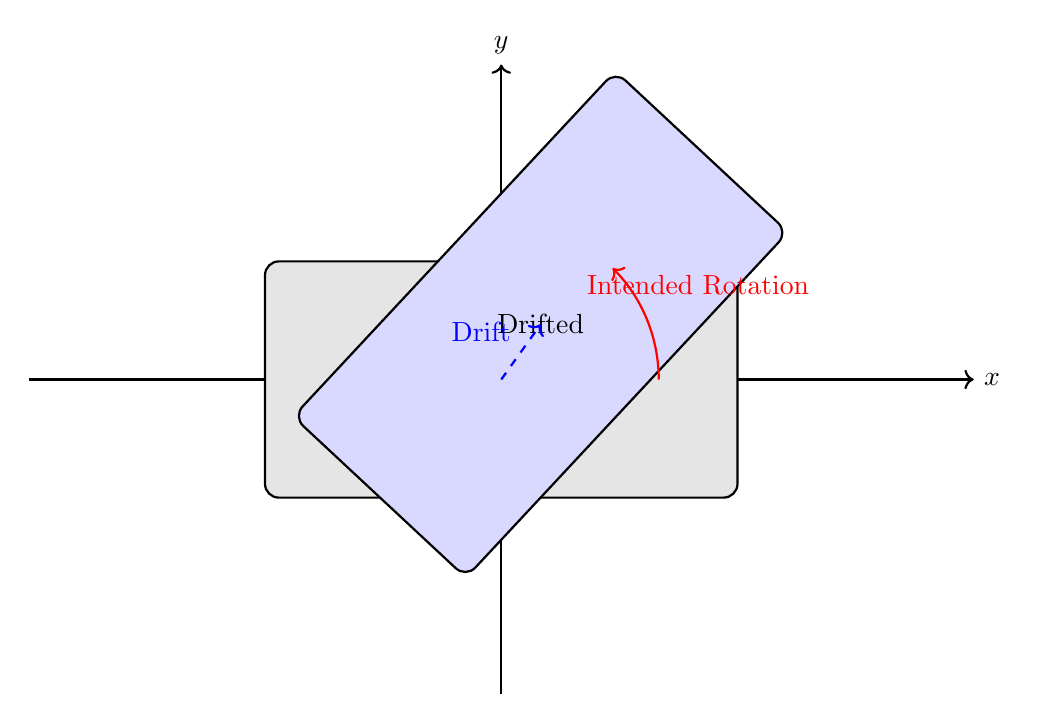
\begin{tikzpicture}[scale=0.1]

    % Axes
    \draw[->, thick] (-60, 0) -- (60, 0) node[right] {$x$};
    \draw[->, thick] (0, -40) -- (0, 40) node[above] {$y$};

    % Original robot (centered at origin)
    \draw[thick, rounded corners=5pt, fill=gray!20]
        (-30, -15) rectangle (30, 15);
    \node at (0, 0) {Initial};

    % Origin marker
    \filldraw[black] (0, 0) circle (0.8);

    % Rotated + drifted robot
    \begin{scope}[shift={(5,7)}, rotate=47] % 45 deg intended + 2 deg yaw drift
        \draw[thick, rounded corners=5pt, fill=blue!15]
        (-30, -15) rectangle (30, 15);
        \node at (0, 0) {Drifted};
    \end{scope}

    % Show rotation arc
    \draw[->, thick, red]
        (20,0) arc[start angle=0, end angle=45, radius=20];
    \node[red] at (25,12) {Intended Rotation};

    % Show drift arrow
    \draw[->, thick, blue, dashed]
        (0,0) -- (5,7) node[midway, above left] {Drift};

    \end{tikzpicture}



    \subsubsection*{Experimental Procedure}

    Two main experiments were designed: one for testing linear forward motion and the other for in-place rotation. In the linear movement test, the robot was commanded to travel forward by a set distance, while in the rotation test, the robot was commanded to rotate by a fixed angle (e.g., 90°). Each command was executed at different speed settings to observe whether error behavior varied with velocity.

    Each experiment was repeated 20 times to ensure statistical significance and to detect any patterns of consistency or randomness in the errors. Measurements of the actual displacement and orientation were obtained using external references (e.g., floor markings or video tracking), and compared against the internal odometry values reported by the robot.

    \subsubsection*{Experiment Configurations}

    \begin{table}[H]
    \centering
    \begin{tabular}{|c|c|c|c|}
    \hline
    \textbf{Test ID} & \textbf{Type} & \textbf{Speed (m/s or rad/s)} & \textbf{Target (m or deg)} \\
    \hline
    L1 & Linear & 0.2 m/s & 1.0 m \\
    L2 & Linear & 0.4 m/s & 1.0 m \\
    L3 & Linear & 0.2 m/s & 0.5 m \\
    R1 & Rotation & 0.5 rad/s & 90° \\
    R2 & Rotation & 1.0 rad/s & 90° \\
    \hline
    \end{tabular}
    \caption{Summary of movement and odometry test configurations}
    \end{table}

    Each test case involved issuing a velocity command for a precise duration such that the robot would cover the target distance or angle, assuming ideal conditions. The difference between the expected and actual outcomes was used to calculate both positional and orientation errors.

    \subsubsection*{Types of Errors Observed}

    During the experiments, several types of errors were encountered:

    \begin{itemize}
        \item \textbf{Systematic Errors:} These occurred consistently in the same direction or magnitude, such as under-rotation by a fixed angle or consistent overshoot in distance. Causes included calibration mismatches, wheel radius misestimation, or delay in motor response.
        
        \item \textbf{Random Errors:} Small variations due to factors like sensor noise, surface friction inconsistencies, or transient slippage. These were not consistent across trials and contributed to spread in the results.

        \item \textbf{Proportional Errors:} Errors that scaled with speed or distance, such as increasing overshoot at higher speeds. This suggested control loop latency or imperfect motor linearity.

        \item \textbf{Fixed Offsets:} Some errors were fixed and independent of input command, like a consistent 2 cm drift to one side. These often pointed to physical asymmetries or encoder misalignments.

        \item \textbf{Odometry Drift:} Over longer trials or repeated motion without reset, odometry drift became more apparent, particularly in rotational tracking.
    \end{itemize}

    \subsubsection*{Correction Strategies}

    To address the errors above, multiple correction strategies were explored:

    \begin{itemize}
        \item \textbf{PID Control:} Implementing a PID loop helped reduce overshoot and improve convergence during both linear and rotational motion. Negative feedback from odometry or external position estimates was used to dynamically adjust motor outputs.

        \item \textbf{Calibration:} Careful calibration of wheel radius, wheelbase, and encoder resolution helped reduce systematic errors.

        \item \textbf{Compensation Factors:} Where errors were consistent and repeatable, simple scalar correction factors were applied post hoc to odometry readings.

        \item \textbf{Sensor Fusion:} Although not implemented in this basic test, more advanced setups could integrate IMUs or vision-based SLAM for odometry correction and drift reduction.

        \item \textbf{Averaging Trials:} For random noise, statistical averaging over multiple trials helped establish a more reliable error profile.
    \end{itemize}

    These experiments form the foundation for understanding the motion characteristics of the YouBot and inform future work in navigation, localization, and control refinement.
    \pagebreak

    \begin{figure}[H]
        \centering
        %/flushleft
        %/flushright
        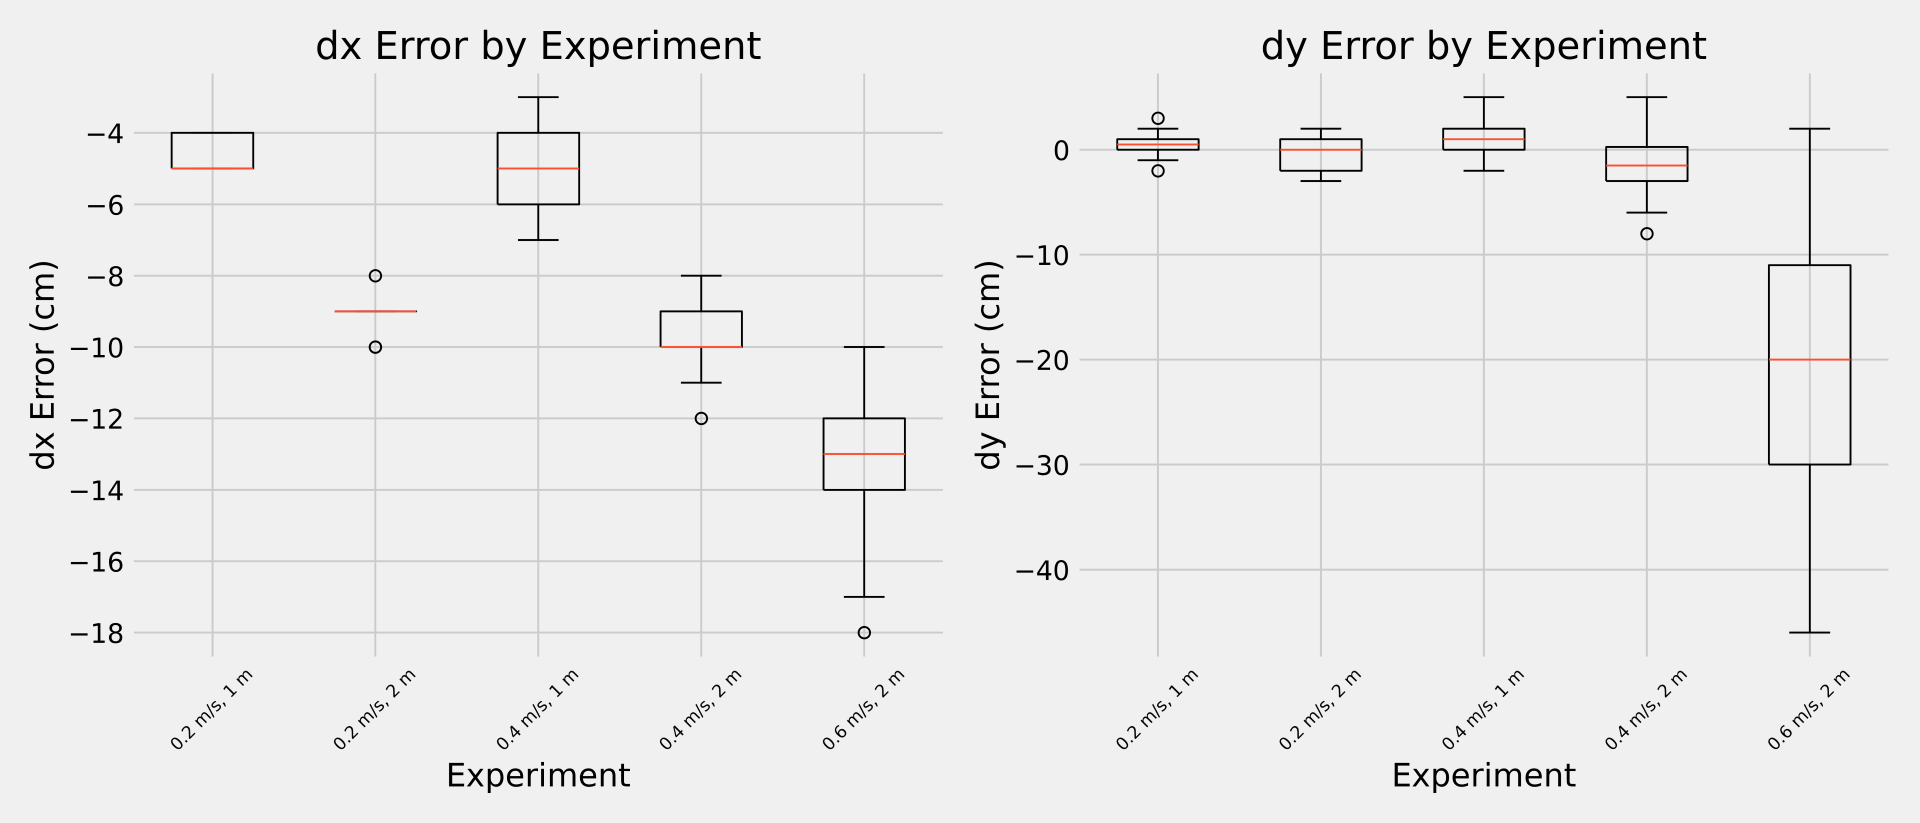
\includegraphics[width=0.99\linewidth]{images/experiment_results/linear_error_boxplots.png}
        \caption{Centered image}
    \end{figure}
    \begin{figure}[H]
        \centering
        %/flushleft
        %/flushright
        
\includegraphics[width=0.99\linewidth]{images/experiment_results/rotational_errors_speed_45.png}
        \caption{Centered image}
    \end{figure}
    \begin{figure}[H]
        \centering
        %/flushleft
        %/flushright
        
\includegraphics[width=0.99\linewidth]{images/experiment_results/rotational_errors_speed_75.png}
        \caption{Centered image}
    \end{figure}

    \pagebreak

    \section{Future Applications}

    In this section we will discuss a potential future application of the KUKA YouBot, in the context of the T\&R method of navigation. The T\&R method is a form of visual SLAM, where the robot can be "taught" a path through a static environment using a camera. The robot then uses this information to enable it to repeat the path movement autonomously through key frames it has saved from the environment. This method is simple yet effective in its use cases and can be used in a variety of applications, such as industrial automation, home robotics, service, etc.

    t\&r is not the best implementation of the youbot
    
    platform and real world application

    why im a bit skeptical about 
    trying to implement t\&r in the context of assistive platform 
    trying to present as an application as a playform that can later on be used to execute repetitive task based on the experience of a platform with 

    speculative : presenting it in terms of real-world applications

    flexible intra-logistics
    human awareness and flexibility 
    seamless human-robot existence

    While the YouBot holds the potential capabilities for undertaking Teach and Repeat, its abilities as a mobile industrial robot base would be better suited for real-world applications within closed environments as an assistive platform. 

    This robot base would be most useful in an assisstie  sense, where it assists humans in completing rather basic and repetitive tasks, like fetching beer. 

    The KUKA YouBot, with its omnidirectional mobile base, offers a flexible platform for experimentation and prototyping in robotics. While the Teach and Repeat (T\&R) method---where a robot is ``taught'' a path using visual cues and then autonomously repeats it---has proven effective in certain domains, its real-world utility as a navigation strategy for assistive platforms is nuanced and context-dependent.

    \subsection{Potential Use Cases for the YouBot Mobile Base}

    The YouBot's mobile base, independent of its manipulator arm, is particularly well-suited for:

    \begin{itemize}
        \item \textbf{Flexible Intra-Logistics:} The YouBot can transport materials, components, or finished goods within factories or laboratories, adapting to dynamic layouts and avoiding obstacles thanks to its omnidirectional drive system. This makes it valuable for automating repetitive transport tasks in manufacturing, electronics, and pharmaceutical environments~.
        \item \textbf{Assistive Service Robotics:} In assistive roles, the mobile base could help with tasks such as fetching objects (e.g., drinks, tools), delivering supplies, or guiding people in structured indoor environments. Such applications are particularly relevant in healthcare, offices, or smart homes, where repetitive, low-complexity tasks can be offloaded from humans to robots~.
        \item \textbf{Research and Prototyping Platform:} The YouBot is widely used in academic and industrial research for developing and testing navigation, mapping, and multi-robot coordination algorithms. Its open interfaces and modular design make it ideal for experimentation in logistics, navigation, and human-robot interaction~.
        \item \textbf{Quality Control and Inspection:} The platform can be equipped with sensors or cameras to autonomously inspect products, monitor environments, or perform routine checks in hazardous or hard-to-reach areas~.
    \end{itemize}

    \subsection{Teach and Repeat (T\&R) in Context}

    The T\&R method, while simple and robust for repeated path following in static environments, has limitations when applied to assistive platforms:

    \begin{itemize}
        \item \textbf{Limited Flexibility:} T\&R excels in environments where the path and surroundings are relatively unchanging. In dynamic or human-populated spaces, its lack of real-time adaptability can be a drawback compared to more advanced SLAM or AI-based navigation systems.
        \item \textbf{Suitability for Repetitive Tasks:} For repetitive, well-defined routes---such as material delivery within a warehouse, or routine inspection rounds---T\&R can be a practical, low-compute solution. However, its application as a general-purpose assistive platform is more speculative, especially where human interaction and environmental variability are significant.
        \item \textbf{Platform Capabilities:} The YouBot's mobile base is robust and maneuverable, making it a strong candidate for T\&R-based applications in controlled settings. Its open architecture allows easy integration of additional sensors or navigation modules, enabling researchers to extend beyond T\&R as needed.
    \end{itemize}

    \subsection{Speculative and Emerging Applications}

    Looking forward, the YouBot mobile base could play a role in:

    \begin{itemize}
        \item \textbf{Seamless Human-Robot Coexistence:} As part of smart environments, YouBots could support flexible logistics, on-demand delivery, and collaborative tasks alongside humans, leveraging both T\&R for routine paths and more advanced navigation for dynamic tasks.
        \item \textbf{Education and Training:} Its accessibility and open-source support make it an excellent tool for teaching robotics concepts, prototyping new algorithms, or participating in competitions such as RoboCup@Work.
        \item \textbf{Translational Research:} Innovations and algorithms developed on the YouBot can be scaled up to larger, industrial-grade mobile platforms, facilitating technology transfer from the lab to real-world production lines.
    \end{itemize}

    \subsection{Summary Table: Potential Use Cases for the KUKA YouBot Mobile Base}

    \begin{table}[h!]
    \centering
    \begin{tabular}{|l|p{7cm}|l|}
    \hline
    \textbf{Application Area} & \textbf{Description} & \textbf{Reference} \\
    \hline
    Intra-logistics & Material transport, flexible routing in factories, labs, or warehouses &  \\
    Assistive service robotics & Fetching/delivery tasks, guidance, support in healthcare or home environments &  \\
    Research and prototyping & Testing navigation, SLAM, multi-robot systems, and human-robot interaction & \\
    Inspection and quality control & Autonomous inspection, monitoring, and data collection in industrial or hazardous settings &  \\
    Education and training & Robotics teaching, student projects, and competitions &  \\
    \hline
    \end{tabular}
    \caption{Potential Use Cases for the KUKA YouBot Mobile Base}
    \end{table}

    \subsection{Conclusion}

    While the KUKA YouBot’s mobile base is not the optimal platform for all assistive applications---especially those requiring high flexibility and human awareness---it remains a valuable tool for developing and demonstrating repetitive, structured tasks. Its use in T\&R navigation is best suited for closed, static environments, but its modularity and open architecture allow for broader experimentation and real-world prototyping in logistics, research, and assistive robotics.

    


    \pagebreak

    \section{Reflection}

    \notes{draft 1, 11.05 6pm}

    In this section, I will reflect on the outcomes of this project. This will include an overview of project management practices and planning, alongside my learnings and personal feelings about the project. 

    \subsection{Project Evolution}

    As disccused previously, the initial goal of this project was much more concrete and ambitious, with an ultimate aim of enabling Teach and Repeat on a decade-old robot whilst using something like ROS2 Jazzy. This was simply not feasible with the outdated software and hardware, lack of documentation, my own lack of experience, and the overall time and resource constraints for completing this project. Furthermore, this project was a significant different experience from any other course I have taken in the past.
    
    My initial approach to project management was very linear and straighforward, with the understanding that there would be no hiccups or issues along the way. I had the following time-table in mind: \notes{maybe insert a table showcasing the plan here?} While this was initially rewarding as I made progress in individual tasks (i.e. Kinect camera, booting up computer, static IP, etc.), momentum was quickly lost when it came to integrating these tasks into a cohesive system, through the use of the ROS1-ROS2 bridge. 

    \subsection{AGILE}

    The new mindset I undertook was inspired by the AGILE project management methodology, which takes a much more flexible and iterative approach to project management. While the long-term goals are still important, the focus is on short-term goals and iterations. This allows for a more flexible approach, where the ending goal can be adjusted based on constraints, feedback, and progress. 

    While this also indirectly means that the project may not be concretely completed, it led to a more flexible exploration of the robot's capabilities and limitations. It furthermore relieved me of the pressure of having to complete a specific (and steep) goal, and gave me breathing space to play around with the available components more freely. This was much more rewarding and enjoyable.

    Undertaking this mindset required time and patience, where I had to learn to accept that not everything would go according to plan. It furthermore required me to be more open to feedback, and actively focusing on short-term goals. 

    \subsection{Final Thoughts}

    Overall, despite the various challenges faced, I am very happy with my progress and learning outcomes regarding this project. I was able to successfully revive the KUKA YouBot to a usable state, gain a deeper understanding of the ROS ecosystem, Linux, bash scripting, alongside the various hardware components of the robot. More importantly, I learned to manage projects with the understanding of personal and technical constraints. I'd like to thank my advisor for his provision of a different perspective on the project, explanations of everything and constant patience.  


    \newpage

    \nocite{*}
    \printbibliography

    \newpage

    \appendix


    \section{User Manual for the KUKA YouBot}

    \subsection{
     How to turn on the YouBot
    }

    \subsection{.bashrc recap}

    \subsection{How to run original demos}

    \section{CSVs and code}

    \subsection{CSV files}
    \subsubsection{Linear movement, 0.2m/s, 1m}
    \begin{table}[H]
    \scriptsize
    \begin{tabular}{@{}cccccc@{}}
    \toprule
    \textbf{dx\_meas} & \textbf{dy\_meas} & \textbf{dx\_odom} & \textbf{dy\_odom} & \textbf{dz\_odom} & \textbf{dyaw\_odom} \\ \midrule
    100          & -4           & 96       & -1       & 0        & -0.012     \\
    103          & -2           & 98       & -2       & 0        & -0.012     \\
    102          & -1           & 98       & -3       & 0        & 0.003      \\
    99           & 0            & 95       & -1       & 0        & -0.006     \\
    102          & -2           & 98       & 0        & 0        & -0.013     \\
    100          & -1           & 95       & 0        & 0        & -0.001     \\
    102          & -1           & 98       & 0        & 0        & 0.005      \\
    103          & -2           & 98       & 0        & 0        & 0.005      \\
    104          & -1           & 99       & -1       & 0        & 0.006      \\
    102          & -2           & 97       & 0        & 0        & -0.004     \\
    103          & 0            & 98       & 0        & 0        & -0.010     \\
    104          & -1           & 99       & -1       & 0        & 0.003      \\
    102          & -1           & 98       & -1       & 0        & 0.004      \\
    102          & 0            & 97       & 0        & 0        & 0.002      \\
    100          & 0            & 96       & -1       & 0        & 0.012      \\
    103          & -1           & 98       & 0        & 0        & 0.007      \\
    103          & -1           & 98       & 0        & 0        & 0.003      \\
    100          & -1           & 96       & 0        & 0        & 0.004      \\
    100          & -1           & 96       & 0        & 0        & -0.003     \\
    103          & 0            & 98       & -1       & 0        & 0.008      \\ \bottomrule
    \end{tabular}
    \end{table}

    \subsubsection{Linear movement, 0.2m/s, 2m}
    \begin{table}[H]
    \scriptsize
    \begin{tabular}{@{}cccccc@{}}
    \toprule
    \textbf{dx\_meas} & \textbf{dy\_meas} & \textbf{dx\_odom} & \textbf{dy\_odom} & \textbf{dz\_odom} & \textbf{dyaw\_odom} \\ \midrule
    207                   & 2                     & 198               & -1                & 0                 & 0.012               \\
    204                   & 0                     & 195               & 0                 & 0                 & 0.002               \\
    207                   & 0                     & 199               & 0                 & 0                 & -0.014              \\
    205                   & -1                    & 196               & 0                 & 0                 & 0.001               \\
    206                   & 0                     & 197               & 0                 & 0                 & 0.003               \\
    207                   & 0                     & 198               & 0                 & 0                 & -0.006              \\
    208                   & -2                    & 199               & 0                 & 0                 & 0.000               \\
    208                   & -2                    & 198               & 0                 & 0                 & 0.008               \\
    208                   & 2                     & 199               & 0                 & 0                 & -0.001              \\
    208                   & 1                     & 199               & 0                 & 0                 & 0.009               \\
    205                   & 2                     & 196               & 0                 & 0                 & 0.004               \\
    209                   & 2                     & 200               & 0                 & 0                 & 0.007               \\
    205                   & 1                     & 196               & 0                 & 0                 & 0.000               \\
    206                   & 2                     & 197               & 0                 & 0                 & 0.014               \\
    208                   & -1                    & 199               & 0                 & 0                 & 0.000               \\
    209                   & -2                    & 199               & 0                 & 0                 & -0.013              \\
    207                   & 2                     & 198               & -1                & 0                 & 0.012               \\
    207                   & -2                    & 198               & 0                 & 0                 & -0.008              \\
    207                   & 0                     & 198               & 0                 & 0                 & 0.004               \\
    205                   & 3                     & 196               & 0                 & 0                 & 0.002               \\ \bottomrule
    \end{tabular}
    \end{table}
    

    \subsubsection{Linear movement, 0.4m/s, 1m}
    \begin{table}[H]
    \scriptsize
    \begin{tabular}{@{}cccccc@{}}
    \toprule
    \textbf{dx\_meas} & \textbf{dy\_meas} & \textbf{dx\_odom} & \textbf{dy\_odom} & \textbf{dz\_odom} & \textbf{dyaw\_odom} \\ \midrule
    94                    & 3                     & 88                & 2                 & 0                 & 0.021               \\
    99                    & -2                    & 94                & 3                 & 0                 & -0.005              \\
    101                   & 0                     & 95                & 2                 & 0                 & 0.002               \\
    93                    & 1                     & 88                & 2                 & 0                 & 0.015               \\
    100                   & 0                     & 94                & 2                 & 0                 & 0.019               \\
    100                   & 1                     & 94                & 3                 & 0                 & 0.005               \\
    100                   & 0                     & 97                & 3                 & 0                 & -0.007              \\
    99                    & 0                     & 94                & 2                 & 0                 & 0.012               \\
    102                   & 2                     & 98                & 2                 & 0                 & 0.018               \\
    101                   & 1                     & 96                & 2                 & 0                 & 0.020               \\
    102                   & 3                     & 97                & 2                 & 0                 & 0.011               \\
    97                    & 2                     & 90                & 3                 & 0                 & 0.013               \\
    95                    & 2                     & 90                & 0                 & 0                 & 0.008               \\
    94                    & 2                     & 90                & 0                 & 0                 & 0.007               \\
    103                   & 0                     & 97                & 0                 & 0                 & 0.004               \\
    97                    & -1                    & 92                & 0                 & 0                 & 0.002               \\
    99                    & -1                    & 95                & 0                 & 0                 & -0.003              \\
    96                    & 0                     & 91                & 0                 & 0                 & -0.006              \\
    100                   & -1                    & 96                & 0                 & 0                 & 0.012               \\
    101                   & -1                    & 97                & 0                 & 0                 & -0.005              \\
    94                    & 0                     & 90                & 0                 & 0                 & -0.006              \\ \bottomrule
    \end{tabular}
    \end{table}
    
    \subsubsection{Linear movement, 0.4m/s, 2m}
    \begin{table}[H]
    \scriptsize
    \begin{tabular}{@{}cccccc@{}}
    \toprule
    \textbf{dx\_meas} & \textbf{dy\_meas} & \textbf{dx\_odom} & \textbf{dy\_odom} & \textbf{dz\_odom} & \textbf{dyaw\_odom} \\ \midrule
    204                   & 3                     & 194               & -1                & 0                 & 0.022               \\
    205                   & 3                     & 194               & -2                & 0                 & -0.010              \\
    206                   & 8                     & 196               & 0                 & 0                 & 0.006               \\
    202                   & 5                     & 192               & -1                & 0                 & 0.012               \\
    205                   & -2                    & 195               & -1                & 0                 & 0.012               \\
    206                   & 3                     & 197               & 2                 & 0                 & 0.004               \\
    199                   & 2                     & 190               & 2                 & 0                 & 0.012               \\
    198                   & 3                     & 190               & 2                 & 0                 & 0.000               \\
    200                   & 0                     & 190               & 2                 & 0                 & -0.002              \\
    205                   & 5                     & 196               & 2                 & 0                 & 0.009               \\
    200                   & 6                     & 190               & 3                 & 0                 & 0.005               \\
    206                   & 4                     & 196               & 2                 & 0                 & 0.020               \\
    205                   & 3                     & 196               & 4                 & 0                 & 0.015               \\
    198                   & 6                     & 190               & 3                 & 0                 & 0.008               \\
    207                   & 3                     & 197               & 2                 & 0                 & 0.024               \\
    207                   & 3                     & 197               & 2                 & 0                 & 0.021               \\
    205                   & 5                     & 195               & 3                 & 0                 & 0.004               \\
    207                   & -2                    & 198               & 3                 & 0                 & -0.009              \\
    207                   & 4                     & 195               & 2                 & 0                 & 0.013               \\
    206                   & -1                    & 196               & 4                 & 0                 & 0.004               \\ \bottomrule
    \end{tabular}
    \end{table} 

    \subsubsection{Linear movement, 0.6m/s, 2m}
    \begin{table}[H]
    \scriptsize
    \begin{tabular}{@{}cccccc@{}}
    \toprule
    \textbf{dx\_meas} & \textbf{dy\_meas} & \textbf{dx\_odom} & \textbf{dy\_odom} & \textbf{dz\_odom} & \textbf{dyaw\_odom} \\ \midrule
    197                   & 0                     & 187               & -4                & 0                 & 0.003               \\
    193                   & 1                     & 179               & -7                & 0                 & 0.006               \\
    203                   & 5                     & 190               & -10               & 0                 & 0.002               \\
    200                   & 5                     & 188               & -15               & 0                 & 0.005               \\
    202                   & 3                     & 189               & -20               & 0                 & 0.003               \\
    201                   & 0                     & 188               & -23               & 0                 & 0.003               \\
    194                   & 0                     & 180               & -25               & 0                 & 0.004               \\
    192                   & 4                     & 178               & -30               & 0                 & 0.003               \\
    198                   & 2                     & 186               & 3                 & 0                 & -0.001              \\
    193                   & -2                    & 181               & 0                 & 0                 & 0.007               \\
    201                   & 0                     & 189               & -3                & 0                 & -0.003              \\
    193                   & -2                    & 181               & -8                & 0                 & -0.002              \\
    204                   & 2                     & 191               & -13               & 0                 & -0.007              \\
    201                   & 0                     & 188               & -14               & 0                 & -0.002              \\
    202                   & 1                     & 189               & -17               & 0                 & 0.006               \\
    203                   & 0                     & 190               & -18               & 0                 & -0.001              \\
    192                   & -1                    & 180               & -21               & 0                 & 0.003               \\
    192                   & 2                     & 180               & -24               & 0                 & -0.002              \\
    193                   & 5                     & 180               & -29               & 0                 & 00.003              \\
    195                   & 7                     & 180               & -34               & 0                 & 0.004               \\
    200                   & 5                     & 184               & -38               & 0                 & -0.001              \\
    204                   & 3                     & 186               & -43               & 0                 & 0.006               \\
    201                   & 1                     & 184               & -45               & 0                 & -0.002              \\ \bottomrule
    \end{tabular}
    \end{table}

    \subsubsection{Rotational movement, 45deg/s, 45deg}
    \begin{table}[H]
    \scriptsize
    \begin{tabular}{@{}cccccccc@{}}
    \toprule
    \textbf{dx1\_meas} & \textbf{dy1\_meas} & \textbf{dx2\_meas} & \textbf{dy2\_meas} & \textbf{dx\_odom} & \textbf{dy\_odom} & \textbf{dz\_odom} & \textbf{dyaw\_odom} \\ \midrule
    1                      & -3                     & -2                     & 1                      & 0                 & 0                 & 0                 & 0.683               \\
    1                      & -3                     & -2                     & 1                      & 0                 & 0                 & 0                 & 0.667               \\
    2                      & -4                     & -2                     & 4                      & 0                 & 0                 & 0                 & 0.596               \\
    2                      & -6                     & -5                     & 5                      & 0                 & 0                 & 0                 & 0.554               \\
    2                      & -4                     & -3                     & 3                      & 0                 & 0                 & 0                 & 0.648               \\
    0                      & -3                     & -1                     & 2                      & 0                 & 0                 & 0                 & 0.711               \\
    0                      & -2                     & -2                     & 2                      & 0                 & 0                 & 0                 & 0.726               \\
    0                      & -3                     & -2                     & 1                      & 0                 & 0                 & 0                 & 0.708               \\
    2                      & -4                     & -3                     & 3                      & 0                 & 0                 & 0                 & 0.633               \\
    2                      & -3                     & -2                     & 2                      & 0                 & 0                 & 0                 & 0.656               \\
    1                      & -5                     & -3                     & 1                      & 0                 & 0                 & 0                 & 0.665               \\
    1                      & -4                     & -2                     & 1                      & 0                 & -1                & 0                 & 0.690               \\
    3                      & -7                     & -4                     & 4                      & 0                 & 0                 & 0                 & 0.553               \\
    2                      & -3                     & -2                     & 3                      & 0                 & 0                 & 0                 & 0.663               \\
    2                      & 0                      & -1                     & 1                      & 0                 & 0                 & 0                 & 0.714               \\
    2                      & -4                     & -2                     & 2                      & 0                 & 0                 & 0                 & 0.674               \\
    3                      & -6                     & -2                     & 5                      & 0                 & 0                 & 0                 & 0.559               \\
    3                      & -4                     & -3                     & 4                      & 0                 & 0                 & 0                 & 0.549               \\
    2                      & -4                     & -2                     & 3                      & 0                 & 0                 & 0                 & 0.665               \\
    2                      & -4                     & -2                     & 2                      & 0                 & 0                 & 0                 & 0.666               \\ \bottomrule
    \end{tabular}
    \end{table}

    \subsubsection{Rotational movement, 45deg/s, 90deg}
        % Please add the following required packages to your document preamble:
    % \usepackage{booktabs}
    \begin{table}[H]
    \scriptsize
    \begin{tabular}{@{}cccccccc@{}}
    \toprule
    \textbf{dx1\_meas} & \textbf{dy1\_meas} & \textbf{dx2\_meas} & \textbf{dy2\_meas} & \textbf{dx\_odom} & \textbf{dy\_odom} & \textbf{dz\_odom} & \textbf{dyaw\_odom} \\ \midrule
    3                      & 0                      & -3                     & 0                      & 0                 & 0                 & 0                 & 1.407               \\
    2                      & 0                      & -2                     & 0                      & 1                 & 0                 & 0                 & 1.439               \\
    0                      & 1                      & -1                     & 0                      & 0                 & 0                 & 0                 & 1.476               \\
    3                      & 0                      & -4                     & 1                      & 0                 & 0                 & 0                 & 1.411               \\
    1                      & 0                      & -1                     & 0                      & 0                 & 1                 & 0                 & 1.479               \\
    -1                     & 0                      & -1                     & 0                      & 0                 & 0                 & 0                 & 1.482               \\
    0                      & 1                      & -4                     & 1                      & 0                 & 0                 & 0                 & 1.460               \\
    0                      & 1                      & 0                      & 1                      & 0                 & 0                 & 0                 & 1.487               \\
    1                      & 1                      & -5                     & 1                      & 0                 & 0                 & 0                 & 1.421               \\
    1                      & 1                      & -5                     & 1                      & 0                 & 0                 & 0                 & 1.423               \\
    3                      & 0                      & -3                     & 0                      & 0                 & 0                 & 0                 & 1.464               \\
    1                      & 2                      & -3                     & 1                      & 0                 & 0                 & 0                 & 1.475               \\
    4                      & 1                      & -5                     & 1                      & 0                 & 0                 & 0                 & 1.403               \\
    1                      & 1                      & -3                     & 1                      & 0                 & 0                 & 0                 & 1.474               \\
    3                      & 2                      & -3                     & 2                      & 0                 & 0                 & 0                 & 1.418               \\
    2                      & 1                      & -3                     & 1                      & 0                 & 0                 & 0                 & 1.458               \\
    4                      & 1                      & -6                     & 1                      & 0                 & 0                 & 0                 & 1.368               \\
    3                      & 2                      & -4                     & 1                      & 0                 & 0                 & 0                 & 1.438               \\
    6                      & 0                      & -4                     & 1                      & -1                & 0                 & 0                 & 1.363               \\
    2                      & 1                      & -2                     & 1                      & 0                 & 1                 & 0                 & 1.469               \\ \bottomrule
    \end{tabular}
    \end{table}

    \subsubsection{Rotational movement, 45deg/s, 180deg}
        % Please add the following required packages to your document preamble:
    % \usepackage{booktabs}
    \begin{table}[H]
    \scriptsize
    \begin{tabular}{@{}cccccccc@{}}
    \toprule
    \textbf{dx1\_meas} & \textbf{dy1\_meas} & \textbf{dx2\_meas} & \textbf{dy2\_meas} & \textbf{dx\_odom} & \textbf{dy\_odom} & \textbf{dz\_odom} & \textbf{dyaw\_odom} \\ \midrule
    1                      & 1                      & 1                      & 2                      & -1                & 0                 & 0                 & 3.042               \\
    1                      & 1                      & 1                      & -1                     & -1                & 1                 & 0                 & 2.994               \\
    0                      & 1                      & 0                      & 2                      & -1                & 0                 & 0                 & 3.020               \\
    1                      & 2                      & 1                      & 2                      & -1                & 1                 & 0                 & 3.041               \\
    0                      & -1                     & 0                      & 0                      & 0                 & 0                 & 0                 & 3.060               \\
    0                      & 1                      & 0                      & -3                     & -1                & 0                 & 0                 & 2.967               \\
    0                      & 2                      & 0                      & -3                     & 0                 & 1                 & 0                 & 2.949               \\
    0                      & 0                      & 1                      & 1                      & 0                 & 0                 & 0                 & 3.047               \\
    1                      & 4                      & 3                      & -5                     & 0                 & 1                 & 0                 & 2.918               \\
    0                      & 2                      & 1                      & -2                     & 0                 & 1                 & 0                 & 2.996               \\
    1                      & -3                     & 1                      & 0                      & 1                 & 1                 & 0                 & 3.302               \\
    0                      & 0                      & 0                      & 0                      & 0                 & 0                 & 0                 & 3.022               \\
    0                      & 0                      & 0                      & 0                      & 0                 & 0                 & 0                 & 3.040               \\
    0                      & 0                      & 1                      & 1                      & 1                 & 0                 & 0                 & 3.047               \\
    0                      & 3                      & 0                      & -3                     & 1                 & 0                 & 0                 & 2.980               \\
    1                      & 3                      & 1                      & -3                     & 1                 & 0                 & 0                 & 2.955               \\
    1                      & 0                      & 0                      & 0                      & 1                 & 0                 & 0                 & 3.041               \\
    1                      & 4                      & 1                      & 4                      & 0                 & 0                 & 0                 & 2.909               \\
    0                      & 0                      & 0                      & 0                      & 0                 & 0                 & 0                 & 3.026               \\
    0                      & 3                      & 0                      & -3                     & 0                 & 0                 & 0                 & 2.934               \\ \bottomrule
    \end{tabular}
    \end{table}
    \subsubsection{Rotational movement, 45deg/s, 360deg}

    \begin{table}[H]
    \scriptsize
    \begin{tabular}{@{}cccccccc@{}}
    \toprule
    \textbf{dx1\_meas} & \textbf{dy1\_meas} & \textbf{dx2\_meas} & \textbf{dy2\_meas} & \textbf{dx\_odom} & \textbf{dy\_odom} & \textbf{dz\_odom} & \textbf{dyaw\_odom} \\ \midrule
    2                      & 5                      & 1                      & -4                     & 0                 & 0                 & 0                 & -0.120              \\
    1                      & 4                      & 1                      & -4                     & 0                 & -1                & 0                 & -0.133              \\
    1                      & 5                      & 1                      & -5                     & 0                 & -1                & 0                 & -0.092              \\
    1                      & 6                      & 1                      & -5                     & 0                 & -1                & 0                 & -0.093              \\
    0                      & 5                      & 1                      & -5                     & 0                 & 0                 & 0                 & -0.055              \\
    1                      & 6                      & 1                      & -6                     & 0                 & 0                 & 0                 & -0.086              \\
    0                      & 0                      & 0                      & 0                      & 0                 & -1                & 0                 & -0.213              \\
    0                      & 5                      & 2                      & -5                     & -1                & 0                 & 0                 & -0.092              \\
    1                      & 5                      & 1                      & -5                     & -1                & 0                 & 0                 & -0.103              \\
    0                      & 2                      & 1                      & 0                      & 1                 & -1                & 0                 & -0.196              \\
    1                      & 1                      & 2                      & 0                      & -1                & 0                 & 0                 & -0.195              \\
    0                      & 4                      & 1                      & -4                     & -1                & 0                 & 0                 & -0.101              \\
    0                      & 4                      & 1                      & -3                     & -1                & 0                 & 0                 & -0.133              \\
    1                      & 5                      & 1                      & -5                     & -1                & 0                 & 0                 & -0.093              \\
    1                      & 5                      & 1                      & -5                     & -1                & 0                 & 0                 & -0.089              \\
    1                      & 1                      & 1                      & 1                      & -1                & 0                 & 0                 & -0.220              \\
    1                      & 5                      & 1                      & -5                     & -1                & 0                 & 0                 & -0.101              \\
    0                      & 5                      & 1                      & -6                     & 0                 & -1                & 0                 & -0.044              \\
    1                      & 4                      & 1                      & -4                     & 0                 & -1                & 0                 & -0.013              \\
    0                      & 5                      & 1                      & -4                     & 0                 & -1                & 0                 & -0.111              \\ \bottomrule
    \end{tabular}
    \end{table}

    \subsubsection{Rotational movement, 75deg/s, 45deg}

    \begin{table}[H]
    \scriptsize
    \begin{tabular}{@{}cccccccc@{}}
    \toprule
    \textbf{dx1\_meas} & \textbf{dy1\_meas} & \textbf{dx2\_meas} & \textbf{dy2\_meas} & \textbf{dx\_odom} & \textbf{dy\_odom} & \textbf{dz\_odom} & \textbf{dyaw\_odom} \\ \midrule
    3                      & -5                     & -3                     & 3                      & 0                 & 0                 & 0                 & 0.630               \\
    6                      & -10                    & -6                     & 10                     & 0                 & 0                 & 0                 & 0.370               \\
    4                      & -6                     & -4                     & 5                      & 0                 & 0                 & 0                 & 0.551               \\
    7                      & -10                    & -5                     & 8                      & 0                 & 0                 & 0                 & 0.422               \\
    5                      & -10                    & -6                     & 10                     & 0                 & 0                 & 0                 & 0.416               \\
    5                      & -6                     & -4                     & 6                      & 0                 & 0                 & 0                 & 0.589               \\
    7                      & -11                    & -6                     & 9                      & 0                 & 0                 & 0                 & 0.422               \\
    4                      & -7                     & -3                     & 4                      & 0                 & 0                 & 0                 & 0.546               \\
    3                      & -3                     & -2                     & 3                      & 0                 & 0                 & 0                 & 0.642               \\
    5                      & -9                     & -5                     & 8                      & 0                 & 0                 & 0                 & 0.443               \\
    3                      & -5                     & -4                     & 4                      & 0                 & 0                 & 0                 & 0.590               \\
    6                      & -10                    & -6                     & 9                      & 0                 & 0                 & 0                 & 0.393               \\
    3                      & -7                     & -3                     & 5                      & 0                 & 0                 & 0                 & 0.556               \\
    3                      & -5                     & -2                     & 3                      & 0                 & 0                 & 0                 & 0.609               \\
    3                      & -5                     & -2                     & 2                      & 0                 & 0                 & 0                 & 0.623               \\
    2                      & -4                     & -3                     & 3                      & 0                 & 0                 & 0                 & 0.594               \\
    3                      & -6                     & -4                     & 3                      & -1                & 0                 & 0                 & 0.585               \\
    2                      & -3                     & -2                     & 3                      & 0                 & 0                 & 0                 & 0.650               \\
    2                      & -3                     & -2                     & 3                      & -1                & 0                 & 0                 & 0.623               \\
    2                      & -3                     & -2                     & 3                      & -1                & 0                 & 0                 & 0.658               \\ \bottomrule
    \end{tabular}
    \end{table}

    \subsubsection{Rotational movement, 75deg/s, 90deg}

    \begin{table}[H]
    \scriptsize
    \begin{tabular}{@{}cccccccc@{}}
    \toprule
    \textbf{dx1\_meas} & \textbf{dy1\_meas} & \textbf{dx2\_meas} & \textbf{dy2\_meas} & \textbf{dx\_odom} & \textbf{dy\_odom} & \textbf{dz\_odom} & \textbf{dyaw\_odom} \\ \midrule
    4                      & 0                      & -6                     & 0                      & 0                 & 0                 & 0                 & 1.346               \\
    11                     & 2                      & -10                    & 1                      & 0                 & -1                & 0                 & 1.205               \\
    1                      & 0                      & -2                     & 0                      & 0                 & -1                & 0                 & 1.437               \\
    -1                     & -2                     & 0                      & 0                      & 0                 & -1                & 0                 & 1.460               \\
    0                      & -1                     & 0                      & 1                      & 0                 & -1                & 0                 & 1.445               \\
    0                      & 6                      & 1                      & -5                     & 0                 & -1                & 0                 & 1.341               \\
    4                      & -1                     & -3                     & 0                      & -1                & -1                & 0                 & 1.415               \\
    2                      & 0                      & -2                     & 0                      & 0                 & -1                & 0                 & 1.464               \\
    3                      & 1                      & -3                     & 1                      & 0                 & 0                 & 0                 & 1.426               \\
    4                      & 1                      & -4                     & 1                      & 0                 & -1                & 0                 & 1.394               \\
    10                     & 1                      & -10                    & 2                      & 0                 & 0                 & 0                 & 1.243               \\
    4                      & 0                      & -2                     & 1                      & -1                & -1                & 0                 & 1.422               \\
    3                      & 0                      & 0                      & 0                      & 0                 & -1                & 0                 & 1.477               \\
    5                      & -1                     & -3                     & 1                      & 1                 & 0                 & 0                 & 1.386               \\
    5                      & 0                      & -4                     & 0                      & 0                 & -1                & 0                 & 1.377               \\
    7                      & 1                      & -8                     & 2                      & 1                 & 0                 & 0                 & 1.287               \\
    10                     & -1                     & -8                     & 2                      & 0                 & -1                & 0                 & 1.211               \\
    3                      & 0                      & 0                      & 1                      & 1                 & -1                & 0                 & 1.463               \\
    5                      & 0                      & -2                     & 1                      & 0                 & -1                & 0                 & 1.432               \\
    7                      & -1                     & -2                     & 0                      & 0                 & -1                & 0                 & 1.358               \\ \bottomrule
    \end{tabular}
    \end{table} 
    \subsubsection{Rotational movement, 75deg/s, 180deg}

    \begin{table}[H]
    \scriptsize
    \begin{tabular}{@{}cccccccc@{}}
    \toprule
    \textbf{dx1\_meas} & \textbf{dy1\_meas} & \textbf{dx2\_meas} & \textbf{dy2\_meas} & \textbf{dx\_odom} & \textbf{dy\_odom} & \textbf{dz\_odom} & \textbf{dyaw\_odom} \\ \midrule
    1                      & 8                      & 3                      & -8                     & 1                 & 0                 & 0                 & 2.769               \\
    0                      & 1                      & 0                      & -1                     & 0                 & 0                 & 0                 & 2.991               \\
    0                      & 1                      & 0                      & -1                     & 0                 & 0                 & 0                 & 2.999               \\
    1                      & 0                      & 1                      & 0                      & 1                 & -1                & 0                 & 3.005               \\
    0                      & 1                      & 0                      & 1                      & 0                 & -1                & 0                 & 3.001               \\
    0                      & 1                      & 1                      & 1                      & 0                 & -1                & 0                 & 2.988               \\
    0                      & 0                      & 1                      & 1                      & 0                 & -1                & 0                 & 3.028               \\
    1                      & 2                      & 1                      & -2                     & -1                & 0                 & 0                 & 2.972               \\
    1                      & 3                      & 1                      & -3                     & -1                & 0                 & 0                 & 2.950               \\
    3                      & 7                      & 3                      & -7                     & -1                & 0                 & 0                 & 2.810               \\
    2                      & 10                     & 3                      & -7                     & -1                & 0                 & 0                 & 2.753               \\
    1                      & 1                      & 1                      & -1                     & 0                 & 1                 & 0                 & 2.951               \\
    1                      & 4                      & 1                      & -2                     & 0                 & 1                 & 0                 & 2.959               \\
    1                      & 1                      & 0                      & 0                      & 1                 & 1                 & 0                 & 2.997               \\
    3                      & 7                      & 0                      & 5                      & 1                 & 0                 & 0                 & 2.825               \\
    1                      & 7                      & 3                      & -7                     & -1                & 0                 & 0                 & 2.794               \\
    1                      & 2                      & 1                      & -2                     & -1                & 0                 & 0                 & 2.967               \\
    2                      & 2                      & 2                      & 2                      & -1                & 1                 & 0                 & 3.030               \\
    2                      & 5                      & 1                      & -3                     & -1                & 1                 & 0                 & 2.926               \\
    2                      & 2                      & 1                      & -3                     & 0                 & 1                 & 0                 & 2.961               \\
    3                      & 10                     & 1                      & -8                     & 1                 & 1                 & 0                 & 2.771               \\ \bottomrule
    \end{tabular}
    \end{table}
    \subsubsection{Rotational movement, 75deg/s, 360deg}

    \begin{table}[H]
    \scriptsize
    \begin{tabular}{@{}cccccccc@{}}
    \toprule
    \textbf{dx1\_meas} & \textbf{dy1\_meas} & \textbf{dx2\_meas} & \textbf{dy2\_meas} & \textbf{dx\_odom} & \textbf{dy\_odom} & \textbf{dz\_odom} & \textbf{dyaw\_odom} \\ \midrule
    1                      & -5                     & 2                      & 6                      & 1                 & 0                 & 0                 & -0.394              \\
    1                      & 3                      & 1                      & -2                     & 1                 & 0                 & 0                 & -0.167              \\
    0                      & 3                      & 1                      & 0                      & 1                 & 1                 & 0                 & -0.203              \\
    1                      & 3                      & 3                      & 7                      & 1                 & 0                 & 0                 & -0.370              \\
    1                      & 5                      & 2                      & -2                     & 1                 & -1                & 0                 & -0.136              \\
    0                      & 5                      & 1                      & -3                     & 1                 & -1                & 0                 & -0.122              \\
    1                      & -1                     & 1                      & 3                      & 1                 & -1                & 0                 & -0.305              \\
    1                      & 4                      & 2                      & -4                     & 0                 & -1                & 0                 & 0.141               \\
    1                      & -2                     & 1                      & 4                      & 0                 & -1                & 0                 & -0.321              \\
    2                      & 2                      & 2                      & -2                     & -1                & 1                 & 0                 & -0.191              \\
    1                      & 2                      & 2                      & 0                      & 0                 & -1                & 0                 & -0.213              \\
    1                      & 2                      & 1                      & -2                     & -1                & -1                & 0                 & -0.184              \\
    2                      & 3                      & 3                      & -2                     & -1                & -1                & 0                 & -0.184              \\
    1                      & -4                     & 1                      & 4                      & -1                & 0                 & 0                 & -0.351              \\
    2                      & 3                      & 2                      & -3                     & -1                & 0                 & 0                 & -0.164              \\
    2                      & 3                      & 3                      & -3                     & -1                & 0                 & 0                 & -0.177              \\
    1                      & -4                     & 1                      & 4                      & -1                & 1                 & 0                 & -0.358              \\
    2                      & 4                      & 2                      & -4                     & -1                & 1                 & 0                 & -0.132              \\
    1                      & 5                      & 2                      & -4                     & -1                & 1                 & 0                 & -0.121              \\
    1                      & 3                      & 2                      & -2                     & -1                & 1                 & 0                 & -0.170              \\ \bottomrule
    \end{tabular}
    \end{table}


    \pagebreak
    \subsection{Python Files}
    %\lstinputlisting[language=Python, caption={Full Script}, label={lst:fullscript}]{../code/rotate_graph.py}
    \subsubsection{rotate\_graph.py}
    \lstinputlisting[language=Python, label={lst:fullscript}]{../code/rotate_graph.py}
    \pagebreak
    \subsubsection{linear\_graph.py}
    \lstinputlisting[language=Python, label={lst:fullscript}]{../code/linear_graph.py}
    \pagebreak
    \subsubsection{linear\_test.py}
    \lstinputlisting[language=Python, label={lst:fullscript}]{../code/youbot-files/DSD/src/youbot_control/scripts/linear_test.py}
    \pagebreak
    \subsubsection{rotate\_test.py}
    \lstinputlisting[language=Python, label={lst:fullscript}]{../code/youbot-files/DSD/src/youbot_control/scripts/rotate_test.py}
    \pagebreak
    \subsubsection{simple\_square\_movement.py}
    \lstinputlisting[language=Python, label={lst:fullscript}]{../code/youbot-files/DSD/src/youbot_control/scripts/simple_square_movement.py}
    \pagebreak
    \subsubsection{Tmux automation script} 
    \lstinputlisting[language=Bash, label={lst:fullscript}]{../code/youbot-files/DSD.sh}

\end{document}
